\documentclass[journal]{IEEEtran}
\usepackage[utf8]{inputenc} % Codificación de entrada UTF-8
\usepackage{cite} % Para citaciones
\usepackage{placeins} % Para \FloatBarrier
\usepackage{graphicx} % Para incluir imágenes
\usepackage{float}
\usepackage{amsmath} % Para fórmulas matemáticas
\usepackage{url} % Para manejar URLs
\usepackage{listings}
\usepackage{xcolor}
\usepackage[ruled,vlined]{algorithm2e} % Para pseudocódigo

% Configuración de listings para bash
\lstset{
  language=bash,
  basicstyle=\ttfamily,
  columns=fullflexible,
  frame=single,
  breaklines=true,
  postbreak=\mbox{\textcolor{red}{$\hookrightarrow$}\space},
  backgroundcolor=\color{lightgray!20},
  keywordstyle=\color{blue},
  commentstyle=\color{green},
  stringstyle=\color{red}
}

% Información del documento
\title{\textbf{Hyper-V Manager vs. Microsoft Hyper-V Server: Dos Caras de la Misma Moneda}}
\author{
  Daniel Antonio Casas Soto \\
  \texttt{dcasass@ulasalle.edu.pe} \\
  Arequipa, Perú \\
  Estudiante de Ingeniería de Software \\
  \and - \\
  Bryan David Motta Bedregal \\\\
  \texttt{bmottab@ulasalle.edu.pe} \\
  Arequipa, Perú \\
  Estudiante de Ingeniería de Software \\
  \and - \\
  Andrea del Rosario Velazco Yana \\
  \texttt{avelazcoy@ulasalle.edu.pe} \\
  Arequipa, Perú \\
  Estudiante de Ingeniería de Software \\
  \and - \\
  Enyelbert Anderson Panta Huaracha \\
  \texttt{epantah@ulasalle.edu.pe} \\
  Arequipa, Perú \\
  Estudiante de Ingeniería de Software
}
\date{\today}
 % Puedes dejar esto vacío o incluir una fecha

\begin{document}

\maketitle

\begin{abstract}
In a rapidly digitizing world, digital tools have embraced advanced levels of virtualization to enhance efficiency and flexibility. This study compares two virtualization systems, Hyper-V Manager and Microsoft Hyper-V Server. While initially appearing similar in functionality, this research unveils significant differences in their implementation and standalone performance, exploring how each can offer distinct advantages in various operational contexts.
\end{abstract}

\begin{IEEEkeywords}
Operative System, Hyper-V, Virtualization, advantages
\end{IEEEkeywords}

\section{Introducción}
En un mundo donde la digitalización avanza sin pausa, las herramientas digitales han evolucionado hacia niveles cada vez más profundos de virtualización. Esta investigación se centra en comparar dos sistemas de virtualización: Hyper-V Manager y Microsoft Hyper-V Server. Aunque inicialmente pueden parecer similares en funcionalidad y propósito, exploraremos cómo cada uno ofrece ventajas distintas cuando se utilizan de manera independiente, destacando sus capacidades y flexibilidad en diferentes escenarios operativos.

\section{Análisis Metodológico}
Esta es una sección principal del artículo. Puedes agregar más secciones según sea necesario.


\subsection{Microsoft Hyper-V Server}
Microsoft Hyper-V es una tecnología de virtualización de hipervisor que permite crear y gestionar máquinas virtuales en un entorno Windows. Hyper-V es parte integral de las versiones de servidor de Windows y también está disponible en algunas ediciones de Windows 10 y Windows 11.
\\ \\
El inicio de un entorno virtual con Hyper-V comienza con una plataforma de hardware diseñada para ser compatible con Windows. Debe tener capacidad para operar en 64 bits y estar habilitada para tecnología de virtualización. Instalado sobre la capa de hardware, y abstrayéndolo de futuras máquinas virtuales (VM), se encuentra el hipervisor.\cite{OLZAK20101}
\begin{figure}[htbp]
  \centering
  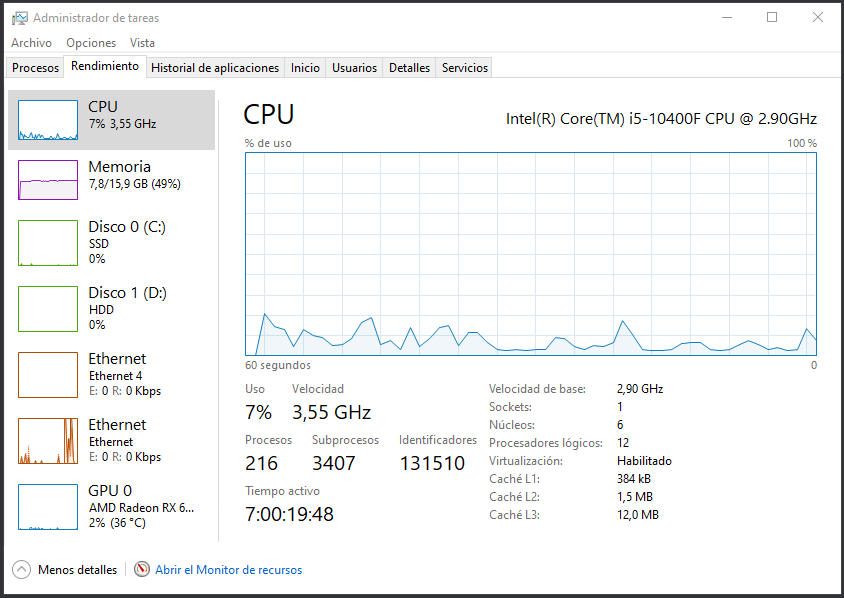
\includegraphics[width=0.3\textwidth]{verificarVirtualizacion.PNG}
  \caption{Verificar si esta habilitado la virtualizacion}
\end{figure}
\\
No todos los procesadores son compatibles con Microsoft Hyper-V. Los procesadores deben soportar la virtualización asistida por hardware (es decir, tecnología Intel VT o AMD-V). 
\begin{figure}[htbp]
  \centering
  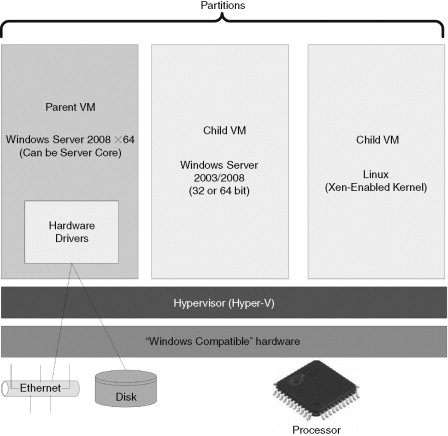
\includegraphics[width=0.3\textwidth]{Hyper V - estructura.jpg}
  \caption{Estructura de Microsoft Hyper-V}
\end{figure}
\\
El hipervisor separa el hardware de los sistemas operativos que se ejecutan en las máquinas virtuales. Configurado y gestionado a través de la VM principal, supervisa los recursos de hardware mediante: 
\\
\begin{itemize}
\item Apoyar la creación y eliminación de máquinas virtuales
\item Administrar el acceso a la memoria y las políticas de seguridad
\item Hacer cumplir las políticas de uso de CPU
\item Programar y gestionar el uso del procesador
\item Gestionar la propiedad de los dispositivos conectados/instalados
\end{itemize}
Las máquinas virtuales en un entorno Hyper-V residen en particiones. La primera partición creada contiene la máquina virtual principal, que debe ejecutar Windows Server 2008 ×64 o Windows Server Core. Una vez que la partición principal esté en operación, se pueden crear particiones secundarias que contengan los entornos de su servidor empresarial.\cite{OLZAK20101}

\subsubsection{Requisitos de Hardware}
\begin{par}
Los requisitos de hardware para Hyper-V no difieren mucho de los requerimientos básicos para Windows Server 2008. Este sistema operativo está disponible en versiones de 32 y 64 bits, mientras que Windows Server 2008 R2 solo está en 64 bits. Sin embargo, Hyper-V solo se encuentra en las ediciones de 64 bits de Windows Server. La CPU debe contar con las extensiones de virtualización necesarias habilitadas en el BIOS. Los principales fabricantes de procesadores, Intel y AMD, ofrecen CPU con estas extensiones.\cite{OLZAK201029}
\begin{figure}[htbp]
  \centering
  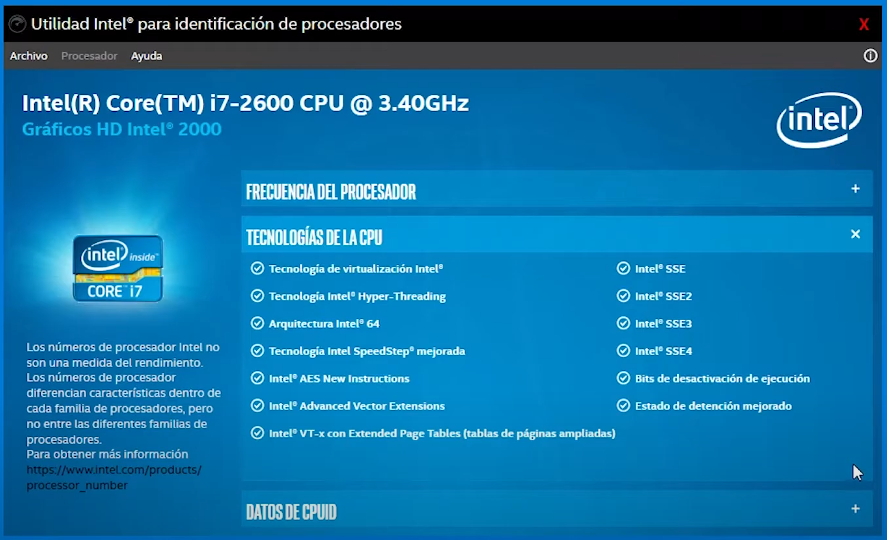
\includegraphics[width=0.3\textwidth]{Comprobacion-Intel.PNG}
  \caption{Comprobar requisitos con procesador Intel}
\end{figure}
\\
La memoria RAM es otro aspecto importante. Además del sistema operativo principal (o "anfitrión"), el sistema operativo virtualizado (o "invitado") también necesita su parte de memoria. Cuantos más sistemas invitados planee ejecutar simultáneamente, más RAM necesitará. Un mínimo recomendado es 4 GB de RAM, ya que esto proporciona suficiente memoria para el invitado y uno o dos anfitriones. No obstante, Microsoft recomienda hasta 8 GB para un rendimiento óptimo.\cite{OLZAK201029}\\ \\
Para el almacenamiento en disco, también debe considerar las necesidades del anfitrión y de cada sistema operativo invitado. En el caso de los invitados, se requiere suficiente espacio en disco para alojar todos los invitados, aplicaciones y datos instalados simultáneamente, independientemente de cuántos se ejecuten al mismo tiempo.\cite{OLZAK201029}\\ \\
Para un rendimiento óptimo, Hyper-V requiere al menos dos adaptadores de red físicos: uno para la gestión del hipervisor y otro para la conectividad de la máquina virtual a la red. Si planea agrupar dispositivos, se recomienda instalar un tercer adaptador.\cite{OLZAK201029}
\end{par}

\subsubsection{Requisitos de software}
Hyper-V está instalado como rol. (Una función es una función predefinida para un servidor, como DNS, Controlador de Active Directory o Hyper-V). Antes de poder instalar la función Hyper-V, debe instalar los paquetes de actualización de Hyper-V para Windows Server 2008 (KB950050 ), así como el paquete de idioma para Hyper-V (KB951636). Hyper-V v2 viene preinstalado en Server 2008 R2; simplemente tienes que habilitarlo. \cite{OLZAK201029}
\subsubsection{Sistemas operativos compatibles con Hyper-V}
Puede instalar sistemas operativos invitados de 32 y 64 bits en Hyper-V. Si bien muchos sistemas operativos pueden instalarse en una instancia de máquina virtual, la siguiente lista cuenta con el respaldo oficial de Microsoft: 
\begin{itemize}
\item Servidor Windows 2000, 2003 y 2008 
\item Servidor empresarial SUSE Linux 10 
\item Windows Vista y Windows 7 Business, Enterprise y Ultimate 
\item Windows XP Profesional
\item Windows 10 Pro, Education
\end{itemize}

\subsection{Hyper-V Manager}

Hyper-V Manager es una herramienta desarrollada por Microsoft que se utiliza para administrar entornos de virtualización en sistemas operativos Windows. Con esta herramienta, los administradores pueden gestionar de manera eficiente máquinas virtuales en servidores y estaciones de trabajo. 
Hyper-V Manager es un complemento de Microsoft Management Console (MMC) que proporciona capacidades administrativas básicas para administrar una o más instancias independientes de Hyper-V. Una de las cosas más comunes con las que luchan los nuevos administradores de Hyper-V es el ecosistema de gestión. No es porque sea un mal ecosistema, sino que se diferencia de las plataformas de la competencia, como VMware, en el sentido de que hay potencialmente cinco interfaces de administración diferentes disponibles, dependiendo del tamaño del entorno que se administra. Analizaremos brevemente cada uno y le mostraremos cuándo entra en juego cada utilidad de administración. \cite{HVM} 
\\ \\
Al permitir la gestión integral de maquinas virtuales también se debe enfatizar que esta capacidad incluye la configuración de aspectos clave como la memoria asignada, los discos duros virtuales y los adaptadores de red. Los administradores pueden realizar operaciones esenciales como iniciar, detener, pausar y guardar el estado de las VMs. Estas funcionalidades aseguran un control total sobre el entorno virtual, permitiendo una gestión precisa y adaptada a las necesidades específicas de cada aplicación.
\\ \\
Una de las características destacadas de Hyper-V Manager es la capacidad de crear snapshots o checkpoints. Estos permiten capturar el estado actual de una máquina virtual, proporcionando un punto de restauración al cual se puede volver en caso de necesidad. Esta funcionalidad es crucial para realizar pruebas y actualizaciones sin riesgo de pérdida de datos. La clonación y exportación de máquinas virtuales son funcionalidades clave que permiten replicar entornos de manera rápida y sencilla. Esto es especialmente útil para la distribución y despliegue de entornos de prueba y desarrollo. Hyper-V Manager soporta la migración en vivo de máquinas virtuales entre diferentes hosts Hyper-V. Esta característica permite trasladar VMs de un host a otro sin interrupción del servicio, asegurando una alta disponibilidad y flexibilidad en la gestión de recursos. Tambien incluye servicios de integración que mejoran la comunicación entre el host y las VMs. Estos servicios permiten la sincronización de tiempo, el intercambio de datos y el apagado seguro de las VMs desde el host. \cite{HVMM}
\\ \\
\begin{figure}
    \centering
    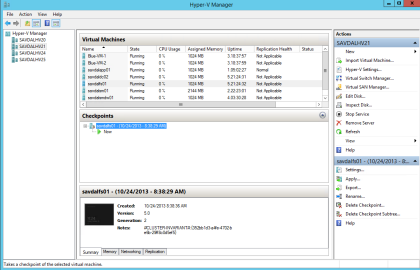
\includegraphics[width=0.3\textwidth]{Interfaz HVM.png}
    \caption{Interfaz de Hyper-V Manager}
\end{figure}
\subsubsection{Requerimientos}
Es compatible con Windows Server y versiones de Windows 10/11 Pro, Enterprise o Education. Estos sistemas operativos ofrecen el soporte necesario para las funcionalidades avanzadas de virtualización que proporciona Hyper-V. \cite{HVMM}
\\
Se requiere un procesador de 64 bits con soporte para la Traducción de Dirección de Segundo Nivel (SLAT), como Intel VT o AMD-V. Este soporte es crucial para la eficiencia y rendimiento de la virtualización, permitiendo a las VMs operar de manera más fluida y con menos sobrecarga de recursos. \cite{HVM}
Se recomienda un mínimo de 4 GB de RAM, aunque la cantidad ideal dependerá de la carga de trabajo y del número de máquinas virtuales que se planea ejecutar simultáneamente. La memoria adecuada asegura que cada VM tenga los recursos necesarios para operar eficientemente.
La virtualización debe estar habilitada en el BIOS/UEFI del sistema. Esta configuración permite que el hardware del sistema soporte plenamente las capacidades de virtualización, mejorando el rendimiento y la estabilidad de las VMs.\cite{HVM}
\\ \\
Hyper-V Manager permite consolidar múltiples servidores virtuales en un menor número de máquinas físicas. Esta consolidación reduce significativamente los costos de hardware y mantenimiento, ya que se necesita menos equipo físico para manejar la misma carga de trabajo. Además, la virtualización permite un uso más eficiente de los recursos, optimizando el rendimiento del hardware existente.

\section{Discusión}
\subsubsection{Hipótesis inicial:}
Dentro de nuestro enunciado inicial, pensamos que Hyper-V Manager, al ser un entorno de virtualización integrado con los servicios de los sistemas operativos Windows Server y Windows Pro/Enterprise, es una opción más adecuada para trabajar en entornos de virtualización. En contraste, Microsoft Hyper-V Server, al ser una versión dedicada exclusivamente a la virtualización y sin un soporte de interfaz gráfica muy robusto, puede presentar dificultades para un programador nuevo que busca herramientas de virtualización distintas a las habituales.\\

Por lo tanto, aunque ambos parezcan tener funcionalidades bastante similares, buscamos verificar las diferencias en funcionalidades y enfoques entre ellos. Estos incluyen el uso de RAM, recursos del sistema y las funcionalidades GUI de las máquinas virtuales creadas. Todos estos puntos nos ayudarán a entender mejor los escenarios específicos en los cuales estos dos entornos de virtualización pueden operar y ser útiles, permitiendo tanto a programadores avanzados como a novatos aprovechar al máximo las capacidades que ofrecen.\\

\subsubsection{Implicaciones del la investigación:}
Para poder ejecutar de la mejor manera este experimento y validar nuestras percepciones previas, seguiremos algunos pasos para realizar pruebas controladas:

\begin{itemize}
    \item Habilitación del sistema de virtualización seleccionado. Esto nos permitirá evaluar la facilidad de instalación en un entorno Windows.
    
    \item Creación de una máquina virtual donde instalaremos una distribución de Linux para verificar las distros soportadas o las que son aceptadas por defecto por el sistema.
    
    \item Instalación de funcionalidades dentro del sistema operativo de la máquina virtual (VM), como g++, gcc, screenfetch y vim; estas herramientas son fundamentales para cualquier programador.
    
    \item Ejecución de un problema de sincronización designado, como el Problema de los filósofos comensales. Esto nos ayudará a evaluar el uso eficiente de hilos y recursos del sistema.
    
    \item Uso de la interfaz gráfica de usuario (GUI) para ejecutar varios programas y evaluar la facilidad y rapidez de uso de la GUI en cada sistema de virtualización.
\end{itemize}

\subsubsection{Consideraciones metodológicas}
En esta sección discutiremos los aspectos metodológicos del estudio presentado para evaluar la robustez y la validez de los hallazgos. En este experimento, se han considerado varios aspectos:

\begin{itemize}
    \item \textbf{Posibles sesgos:} Se ha realizado un esfuerzo consciente por minimizar cualquier sesgo en la selección de la versión de las herramientas de virtualización y en la configuración de las pruebas, puesto que quienes ejecutaron las pruebas usan máquinas diferentes.
    
    \item \textbf{Limitaciones del diseño experimental y factores de hardware:} Aunque se han diseñado pruebas controladas, se reconoce que existen limitaciones inherentes al entorno de virtualización y a la configuración específica utilizada, siendo el caso de la RAM de cada computador usado para las pruebas o la velocidad del procesador; asi como la versión del Windows que se ha utilizado.  
  
    \item \textbf{Evaluación de la reproducibilidad:} Se facilitará la reproducibilidad del experimento mediante la documentación detallada de los pasos y configuraciones utilizadas, asi como imágenes que muestran algunos escenarios esperables para el experimento.
\end{itemize}

Estas consideraciones metodológicas son fundamentales para contextualizar los resultados y permitir una evaluación crítica de la fiabilidad y la aplicabilidad de los hallazgos obtenidos.


\section{Resultados}

\subsection{Instalación y prueba de Hyper-V Manager}
Para instalar Hyper-V Manager tenemos que tener en cuenta que la mayoría de sistemas de Windows tienen ya un acceso garantizado para poder instalar estos sistemas de virtualización.\\
Lo único es que necesitamos es permitir que estos puedan verse permitidos por nuestras varibles de entorno y características del SO. \\
\subsubsection{Habilitación de Hyper-V Manager}
Hyper-V Manager puede ser habilitado desde la consola, el PowerShell o el propio panel de control\cite{Wlear2024}, sin embargo se sugiere que se pueda habilitar por medio de la consola ya que la implementación se vuelve más amigable con el usuario.\\

\begin{figure}[htbp]
  \centering
  \includegraphics[width=0.3\textwidth]{Hyper-V/Instalación 2.png}
  \caption{Habilitando Hyper-V Manager Part.1}
\end{figure}

Tenemos que incluir este comando para poder ''Descargar'' el Hyper-V Manager, así podremos utilizarlo durante nuestro proceso de virtualización, esto lo hacemos abriendo nuestra consola como administrador\cite{Wlear2024} :\\

\begin{lstlisting}[language=bash]
Enable-WindowsOptionalFeature -Online -FeatureName Microsoft-Hyper-V -All
\end{lstlisting}

\begin{figure}[htbp]
  \centering
  \includegraphics[width=0.3\textwidth]{Hyper-V/Instalación 1.png}
  \caption{Habilitando Hyper-V Manager Part.2}
\end{figure}

 Luego podremos ver que terminaremos de habilitar nuestro sistema con el comando de DISM, que es el administrador de imágenes de Windows, más que nada para acomodar el uso de la plataforma de virtualización\cite{Wlear2024} :\\

\begin{lstlisting}[language=bash]
DISM /Online /Enable-Feature /All /FeatureName:Microsoft-Hyper-V
\end{lstlisting}

\subsubsection{Activación de entorno de virtualización:}
Después de haber habilitado todo nuestro entorno de virtualización como sistema, ahora necesitamos activarlo dentro de nuestr SO, esto nos permitirá que Hyper-V Manager tenga los permisos necesarios para ejecutarse dentro de la gestión de imágenes de nuestro Windows.\\

\begin{figure}[htbp]
  \centering
  \includegraphics[width=0.3\textwidth]{Hyper-V/Instalación 3.png}
  \caption{Activando virtualización en nuestra Pc. Part.1}
\end{figure}

\begin{figure}[htbp]
  \centering
  \includegraphics[width=0.3\textwidth]{Hyper-V/Instalación 4.png}
  \caption{Activando virtualización en nuestra Pc. Part.2}
\end{figure}

\begin{figure}[htbp]
  \centering
  \includegraphics[width=0.3\textwidth]{Hyper-V/Instalación 5.png}
  \caption{Activando virtualización en nuestra Pc. Part.3}
\end{figure}

En líneas generales tenemos que ir a programas y características y luego a ''Características de Windows'' para poder habilitar dentro de las nuestro Windows el ''Microsoft Hyper-V'', a pesar que nos parezca igual que el Microsoft Hyper-V server, es la misma habilitación para el Hyper-V Manager\cite{Wlear2024}.\\

\subsubsection{Inicialización de Hyper-V Manager e instalación de Ubuntu 22 (JellyFish):}

Dentro de nuestro esfuerzo por ejecutar pruebas dentro de Hyper-V Manager, necesitamos usar este entorno de virtualización para poder crear una máquina virtual. Esta la haremos de:
\begin{itemize}
    \item Ubuntu 22.04.4 LTS
    \item RAM 2048 MB
    \item 2 Procesadores Virtuales
\end{itemize}
Siguiendo estas especificaciones se procederá a crear la máquina virtual.

\begin{figure}[htbp]
  \centering
  \includegraphics[width=0.3\textwidth]{Hyper-V/Instalación 6.png}
  \caption{Instalación de Ubuntu en nuestra máquina virtual. Part.1}
\end{figure}

\begin{figure}[htbp]
  \centering
  \includegraphics[width=0.3\textwidth]{Hyper-V/Instalación 7.png}
  \caption{Instalación de Ubuntu en nuestra máquina virtual. Part.2}
\end{figure}

\begin{figure}[htbp]
  \centering
  \includegraphics[width=0.3\textwidth]{Hyper-V/Instalación 8.png}
  \caption{Instalación de Ubuntu en nuestra máquina virtual. Part.3}
\end{figure}

\subsubsection{Instalación de Ubuntu 22 (JellyFish), modo usual:}
Luego de elegir nuestro Ubuntu 22, procederemos a instalarlo como se hace usualmente en una PC.\\

\begin{figure}[htbp]
  \centering
  \includegraphics[width=0.3\textwidth]{Hyper-V/Instalación 9.png}
  \caption{Instalación de Ubuntu en nuestra máquina virtual. Part.4}
\end{figure}

\begin{figure}[htbp]
  \centering
  \includegraphics[width=0.3\textwidth]{Hyper-V/Instalación 9.5.png}
  \caption{Instalación de Ubuntu en nuestra máquina virtual. Part.5}
\end{figure}

Con el Ubuntu instalado, haremos algunas pruebas dentro de este, para corroborar el rendimiento de este sistema de virtualización, sin embargo necesitamos ingresar a nuestra máquina virtual para ello tenemos que recordar la contraseña con la que la creamos y el usuario que pusimos\cite{VirtualM}, ya que, luego que la iniciemos necesitaremos iniciar sesión en ''xorg'', este es como un modo mejorado (enhanced) para la seguridad de nuestra Virtual Machine \cite{Xorg}.

\subsubsection{Pruebas en Hyper-V Server:}

Para ejecutar algunas pruebas haremos la instalación de ''gcc, g++, vim y screenfetch''\\

\begin{figure}[htbp]
  \centering
  \includegraphics[width=0.3\textwidth]{Hyper-V/Instalación 10.png}
  \caption{Pruebas en Ubuntu}
\end{figure}

\begin{figure}[htbp]
  \centering
  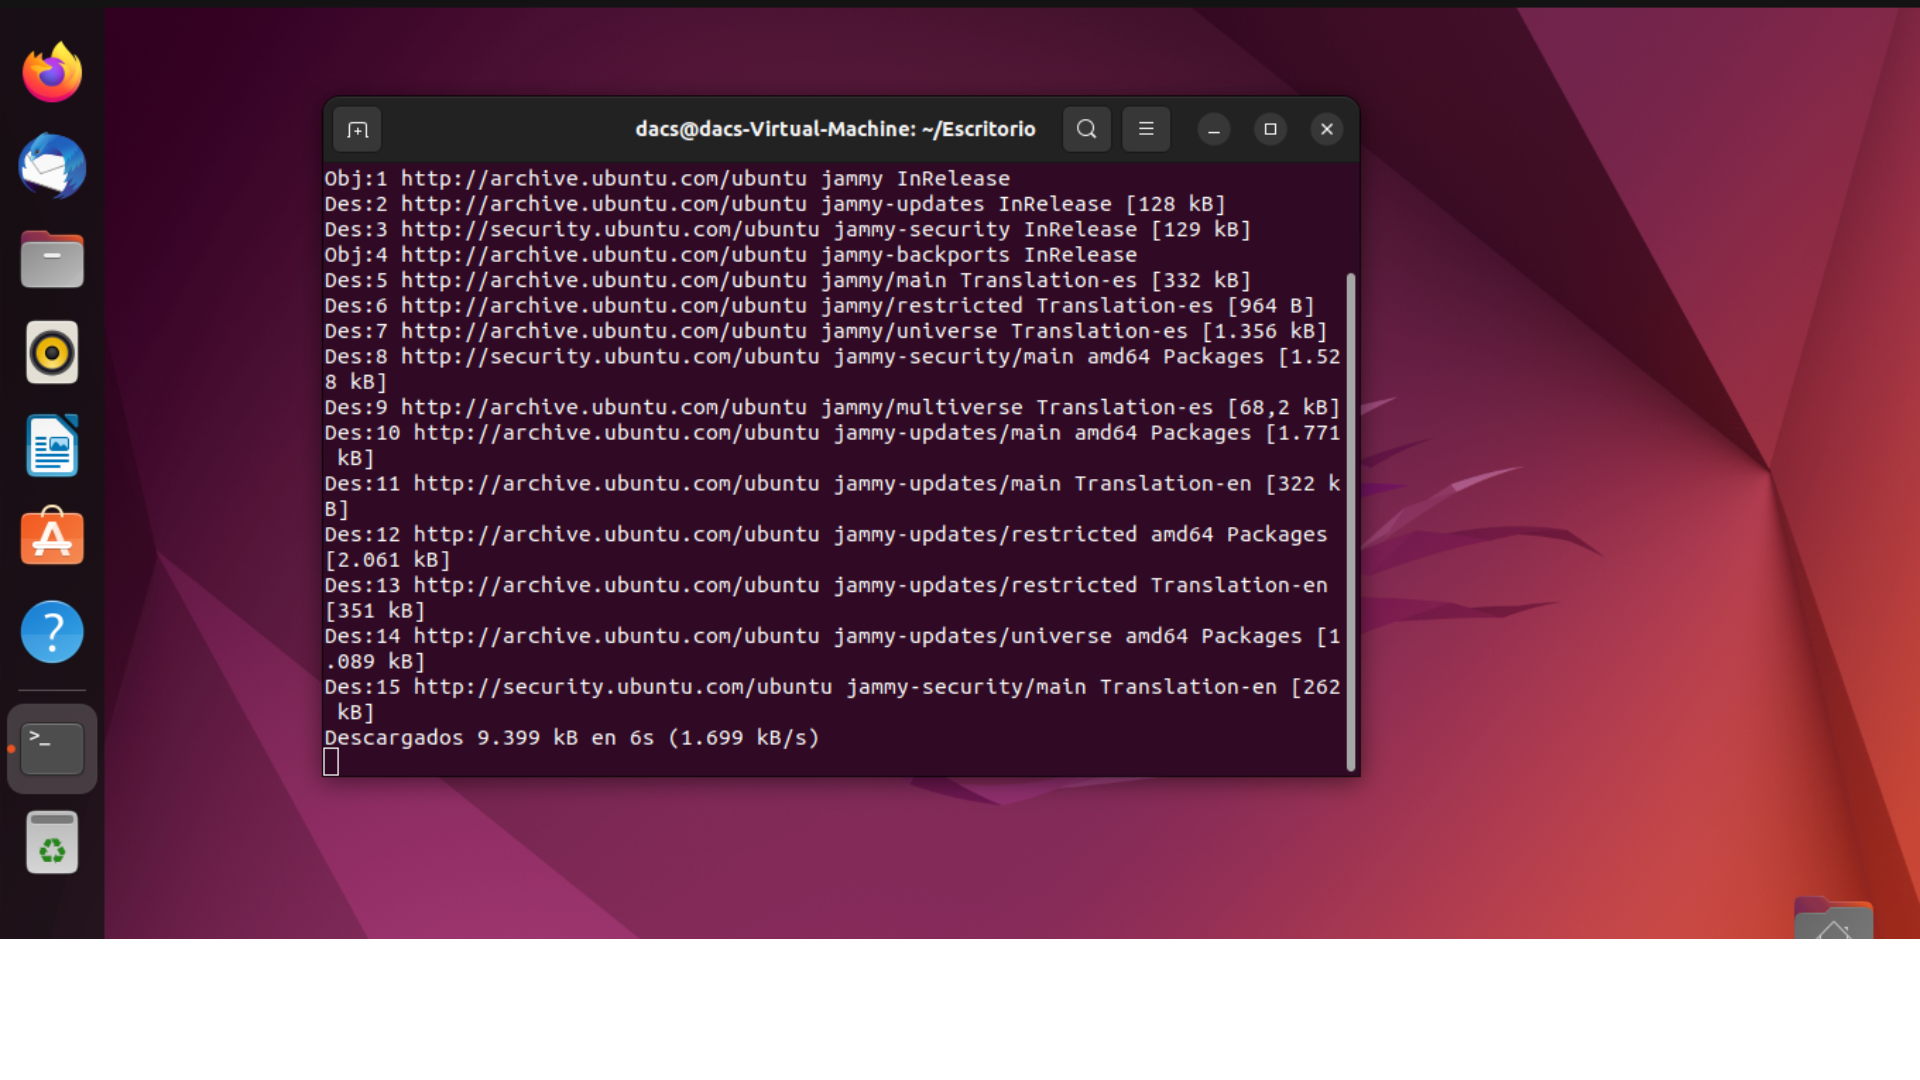
\includegraphics[width=0.3\textwidth]{Hyper-V/1.png}
  \caption{Actualizamos los paquetes de Ubuntu}
\end{figure}

Aquí ejecutaremos el comando para poder actualizar estos paquetes.\\
\begin{lstlisting}[language=bash]
sudo apt update
\end{lstlisting}

\subsubsection{Instalación de gcc, g++, vim y screenfetch:}

Se procederá a instalar por consola los programas requeridos.\\

\begin{figure}[htbp]
  \centering
  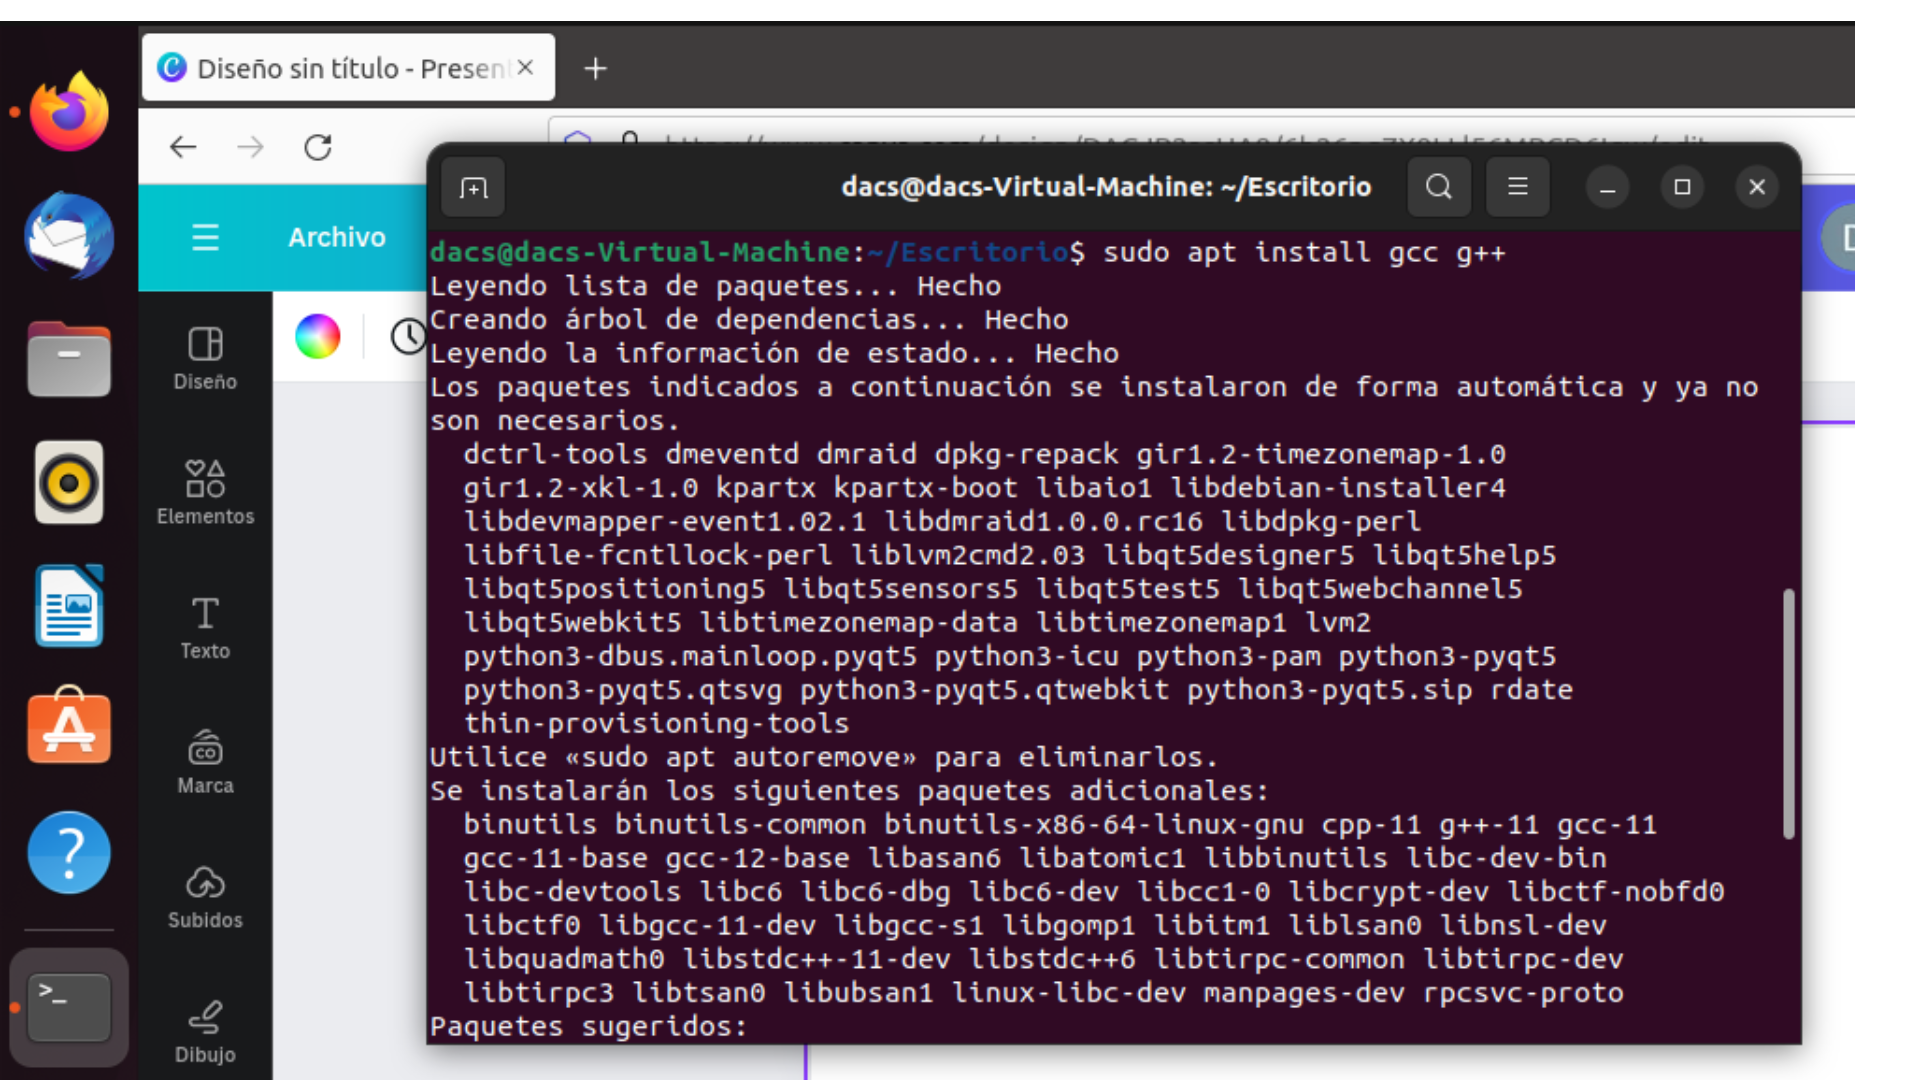
\includegraphics[width=0.3\textwidth]{Hyper-V/2.png}
  \caption{Instalación de gcc y g++}
  \begin{lstlisting}[language=bash]
    sudo apt install gcc g++
  \end{lstlisting}
\end{figure}

\begin{figure}[htbp]
  \centering
  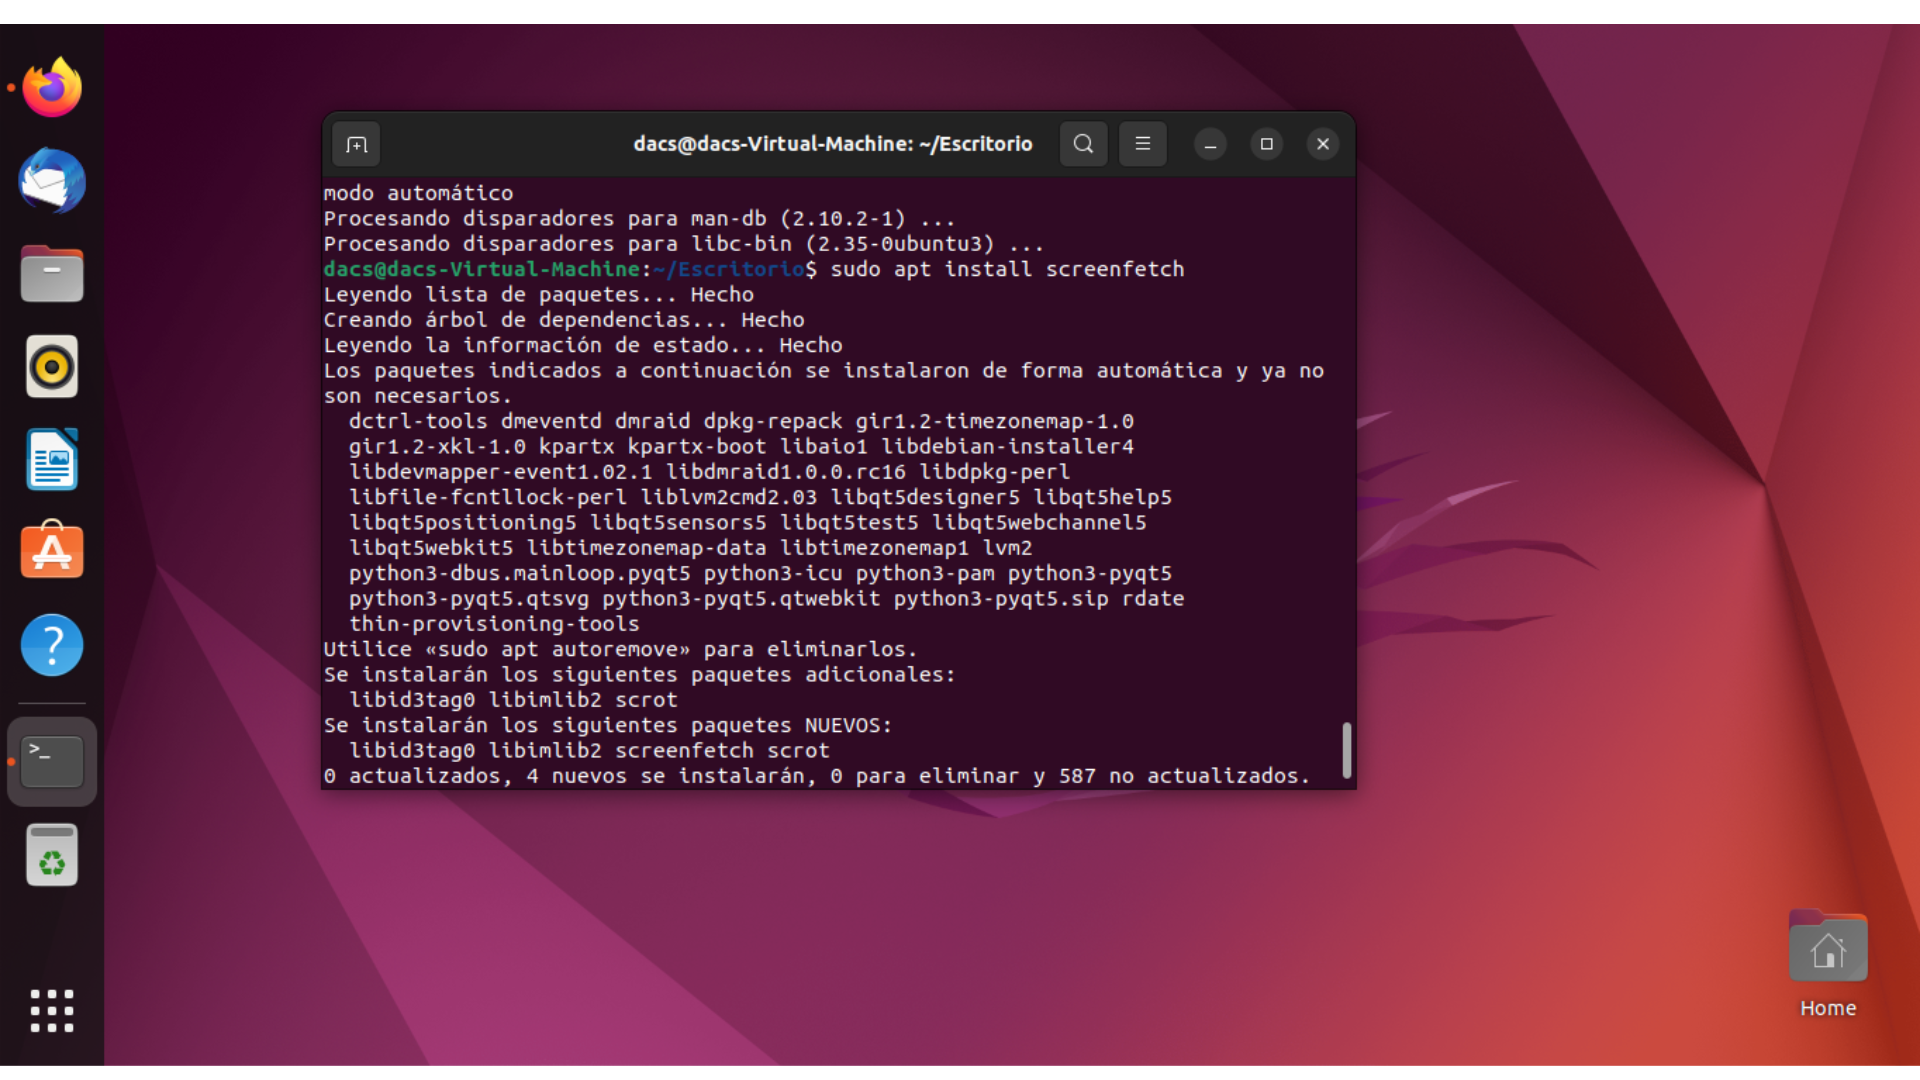
\includegraphics[width=0.3\textwidth]{Hyper-V/3.png}
  \caption{Instalación de screenfetch}
  \begin{lstlisting}[language=bash]
    sudo apt install screenfetch
  \end{lstlisting}
\end{figure}

\begin{figure}[htbp]
  \centering
  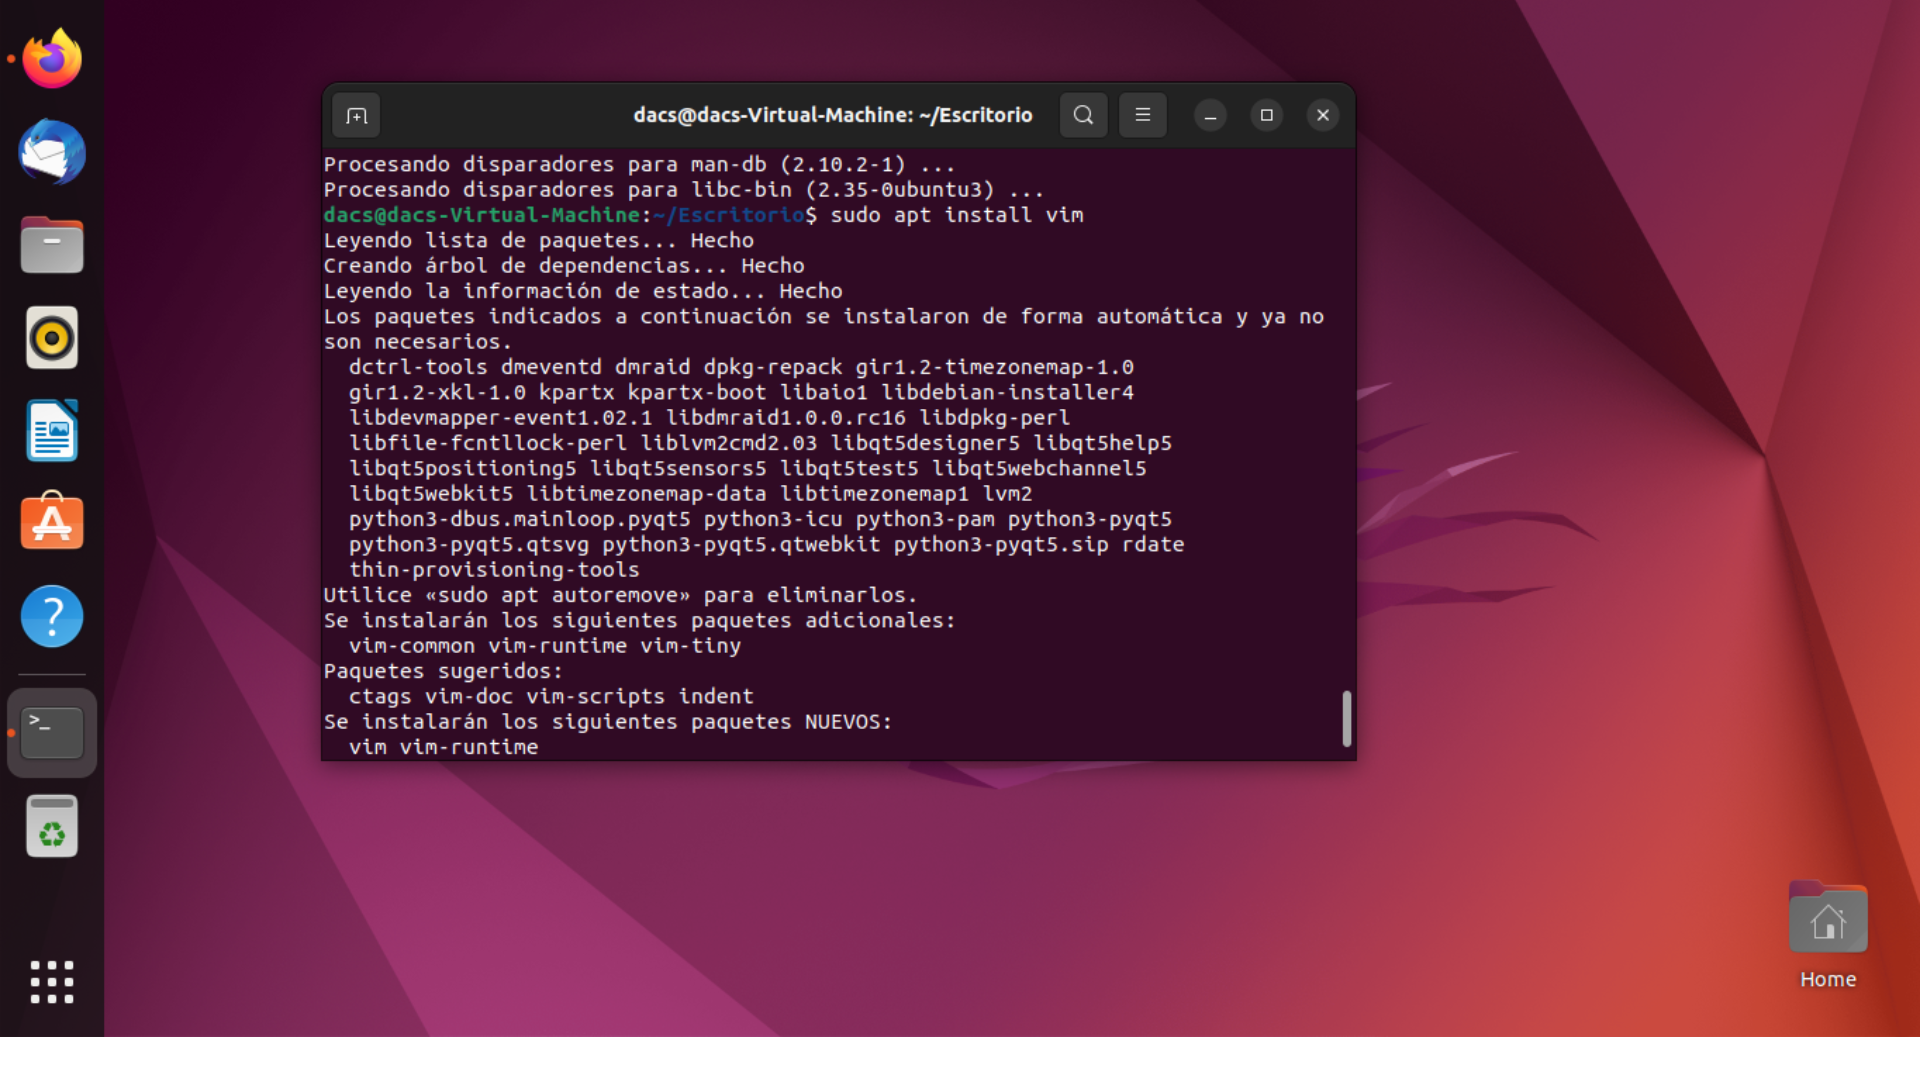
\includegraphics[width=0.3\textwidth]{Hyper-V/4.png}
  \caption{Instalación de vim}
  \begin{lstlisting}[language=bash]
    sudo apt install vim
  \end{lstlisting}
\end{figure}

Luego comprobaremos la instalación correcta de cada uno de estos con los comandos de ejecución de cada aplicación, esto nos servira para saber si se instalaron correctamente y poder tener una ejecución adecuada de nuestro ejemplo de prueba posteriormente.

\begin{figure}[htbp]
  \centering
  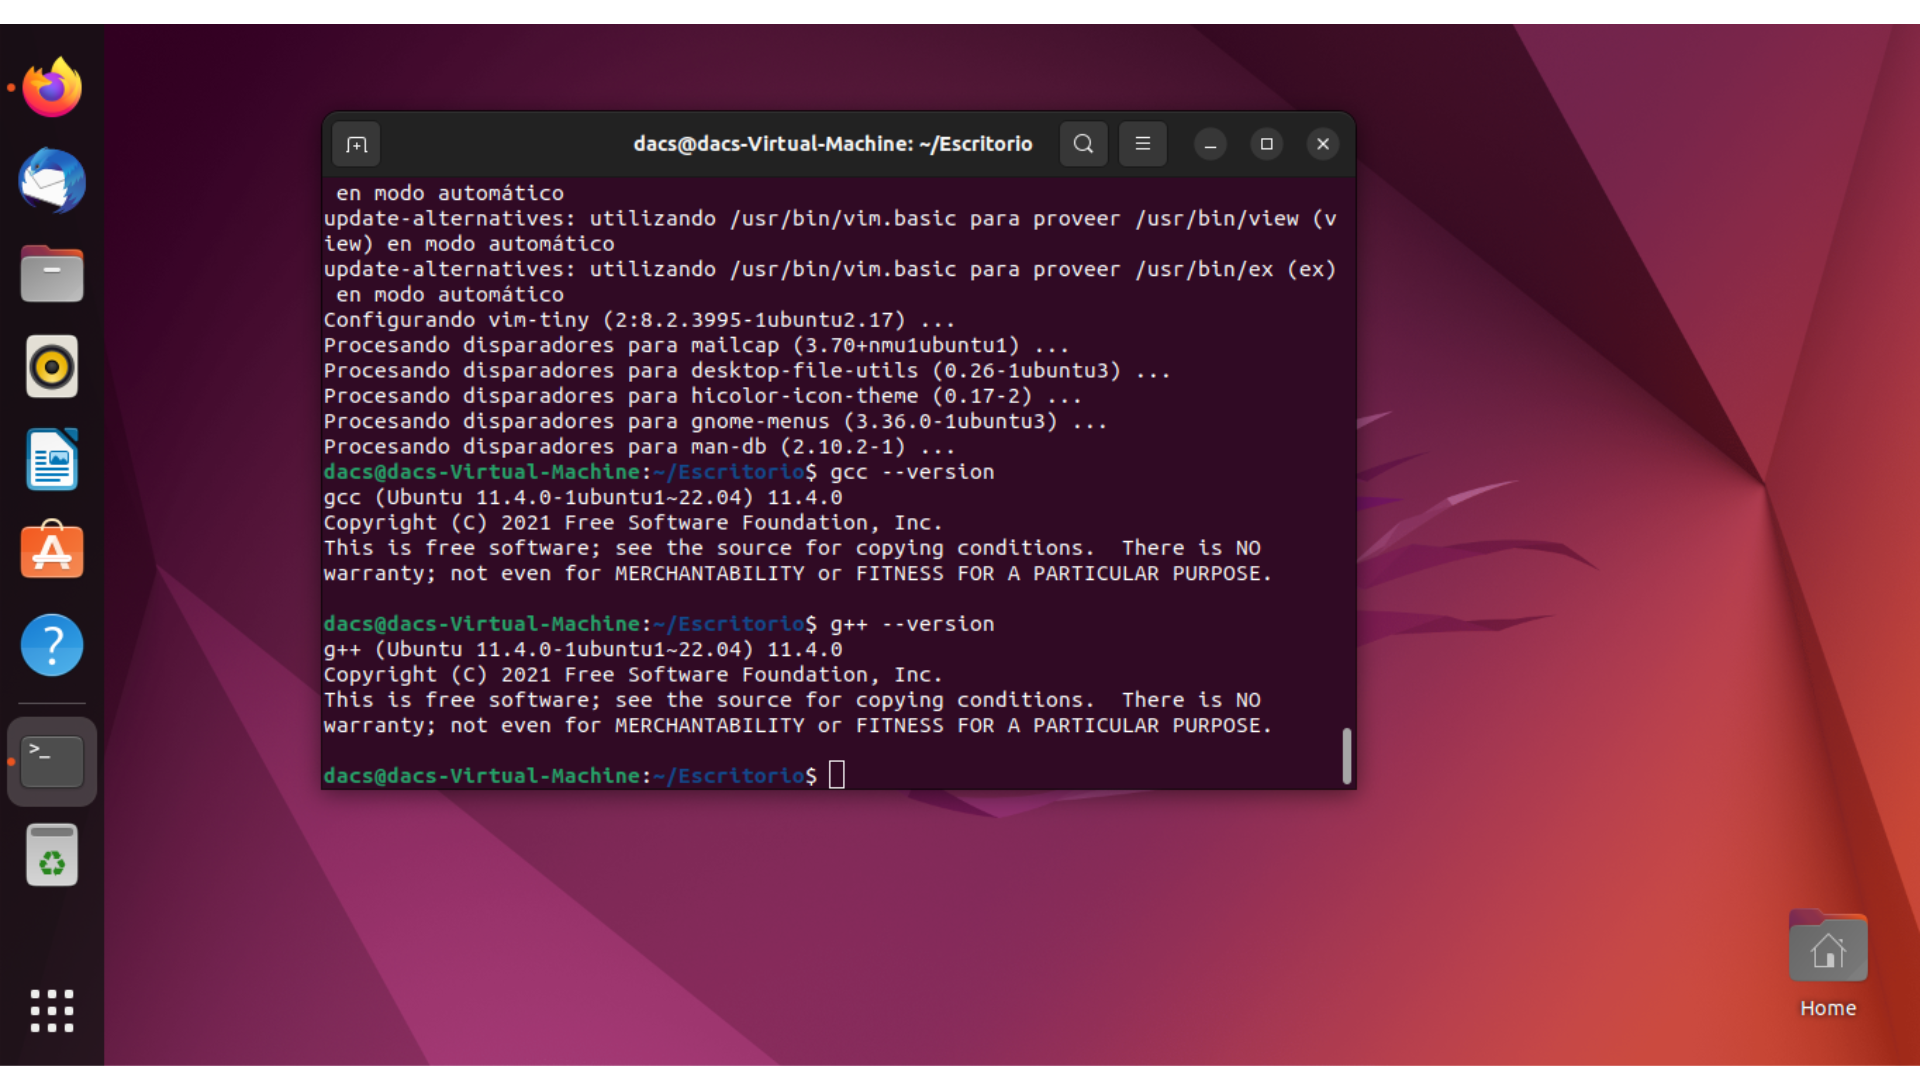
\includegraphics[width=0.3\textwidth]{Hyper-V/5.png}
  \caption{Comprobación de gcc y g++}
  \begin{lstlisting}[language=bash]
    gcc --version
    g++ --version
   \end{lstlisting}
\end{figure}

\begin{figure}[htbp]
  \centering
  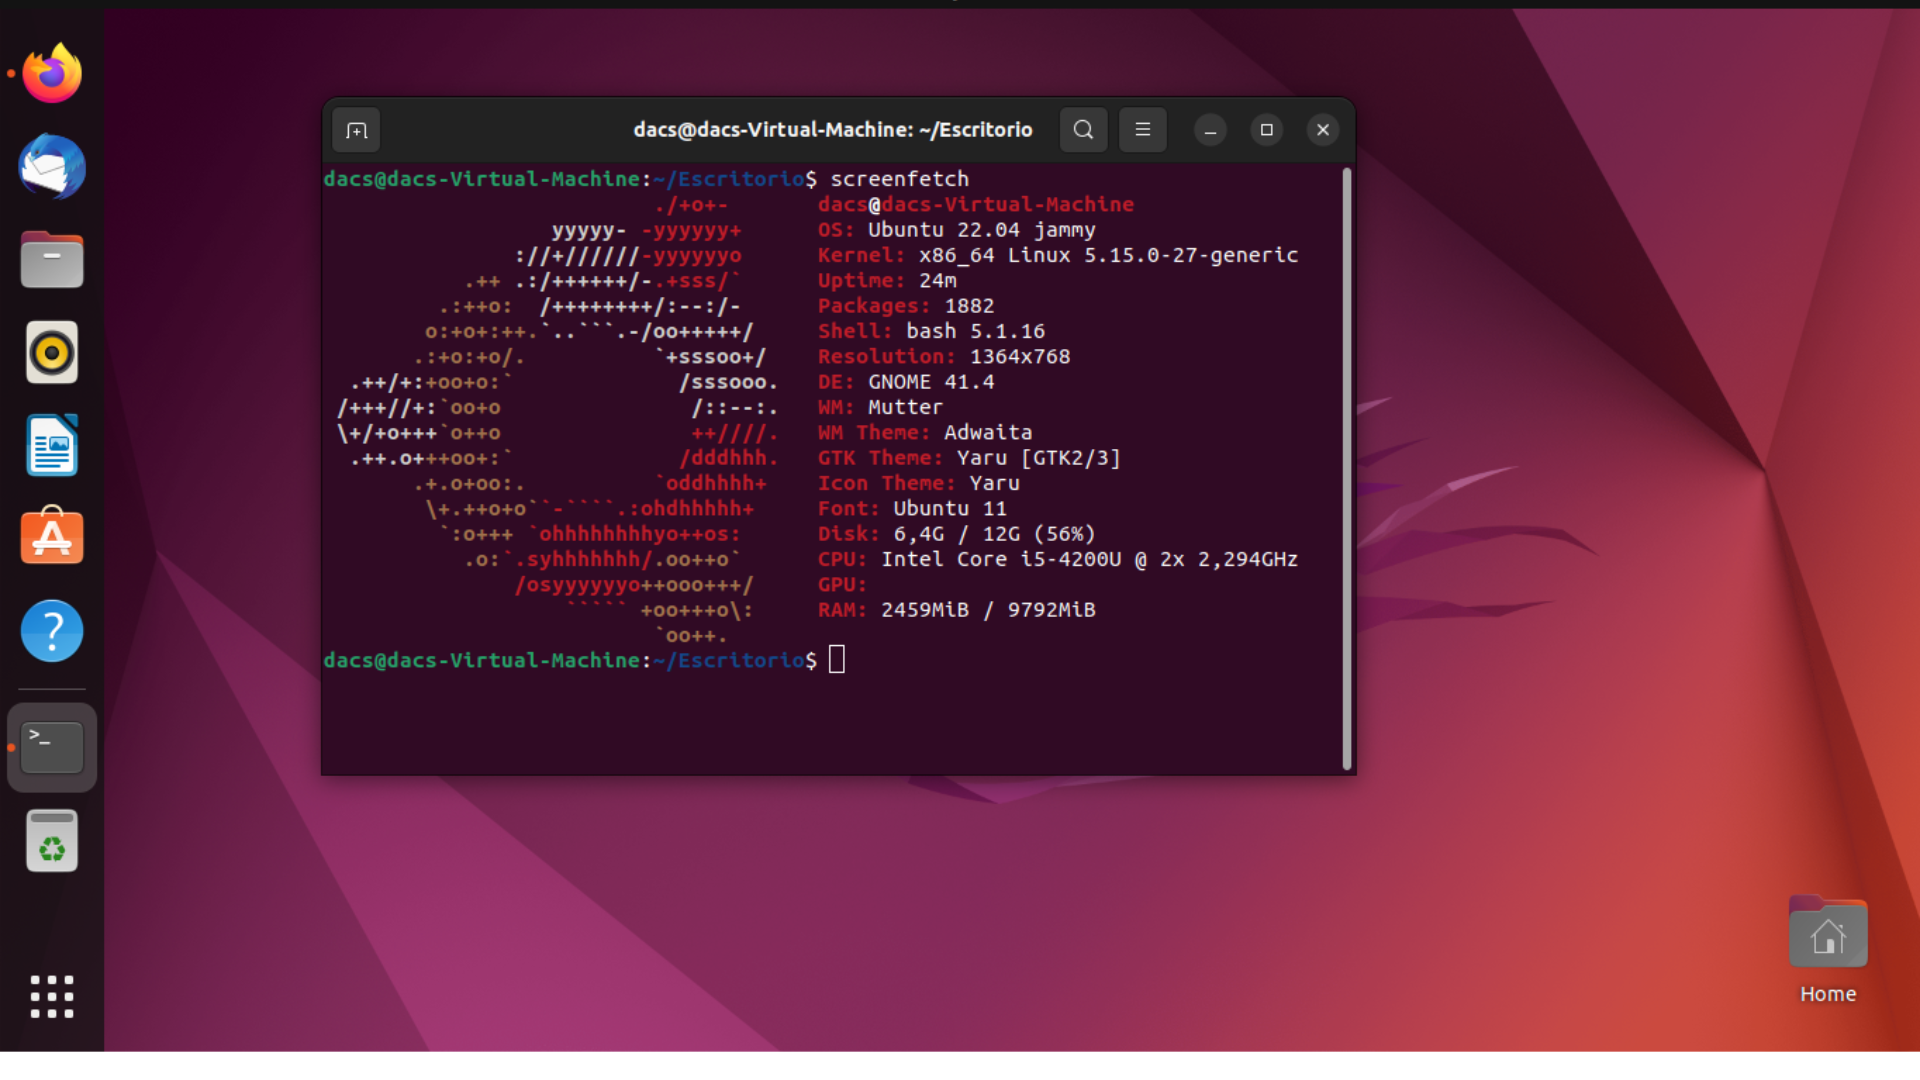
\includegraphics[width=0.3\textwidth]{Hyper-V/6.png}
  \caption{Comprobación de screenfetch}
  \begin{lstlisting}[language=bash]
    screenfetch
  \end{lstlisting}
\end{figure}

\begin{figure}[h!]
  \centering
  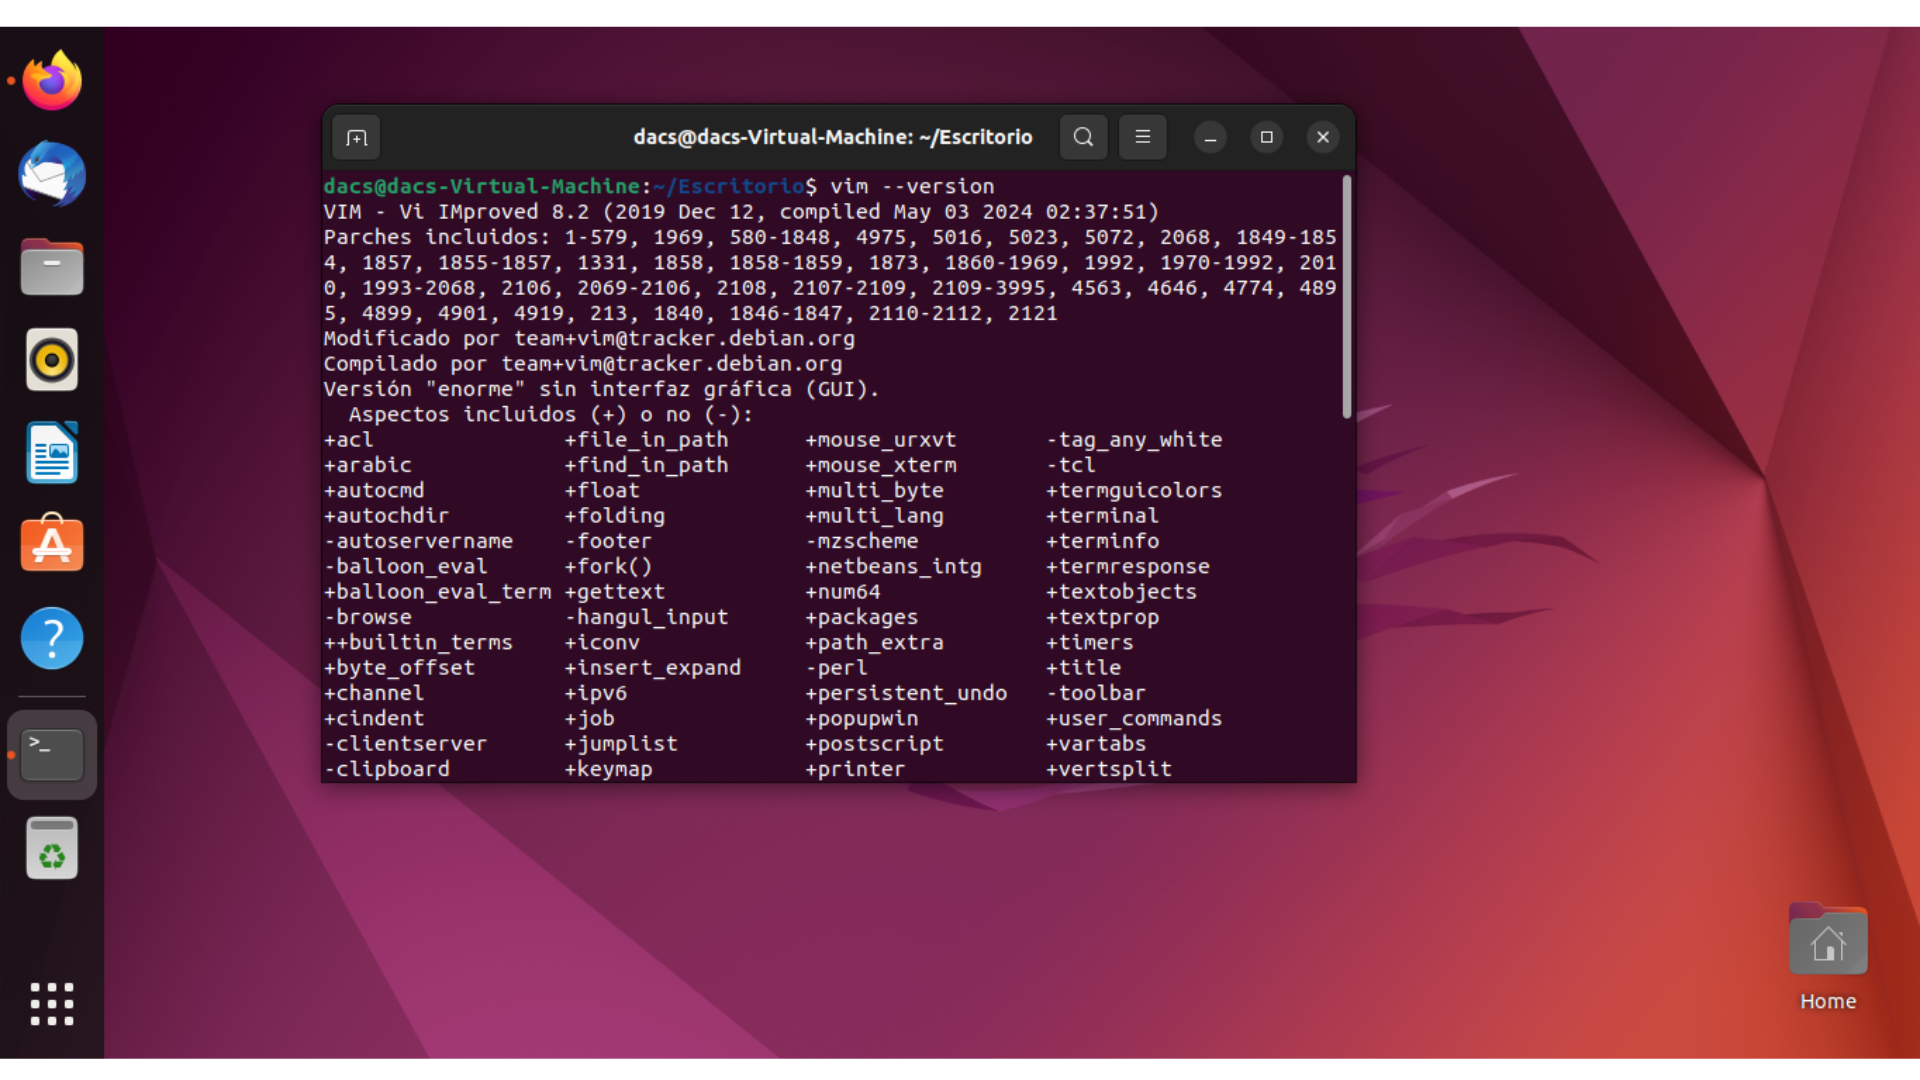
\includegraphics[width=0.3\textwidth]{Hyper-V/7.png}
  \caption{Comprobación de Vim}

  \begin{lstlisting}[language=bash]
    vim --version
  \end{lstlisting}
\end{figure}

\FloatBarrier %Evita que una figura se salga de una sección asignada

\subsubsection{Prueba de hilos y de GUI:}
Para poder probar la eficiencia en el uso de los recursos que se le asignaron a esta máquina virtual, se procederá a ejecutar un código simple del problema de los ''Filosofos comensales'', problema de sincronización anteriormente trabajado, que nos brindará una percepción adecuada del uso de recursos que nos da el sistema, asi mismo, como una sincronización de procesos eficiente para nuestro máquina virtual.\\

Utilizaremos el pseudocódigo investigado \cite{PhiloWiki}, para poder ejecutar un ejemplo de este problema en nuestro entorno virtual.

\begin{algorithm}[H]
\SetAlgoLined
\KwData{tenedores[5], estado\_filosofos[5]}
\KwResult{Gestión de filósofos comiendo y pensando}
\SetKwFunction{FnCambiarEstado}{cambiar\_estado}
\SetKwFunction{FnEstadoIzquierdo}{estado\_izquierdo}
\SetKwFunction{FnEstadoDerecho}{estado\_derecho}
\SetKwFunction{FnIntentarComer}{intentar\_comer}
\SetKwFunction{FnDejarComer}{dejar\_comer}
\SetKwFunction{FnFilosofo}{filosofo}
\SetKwFunction{FnPensar}{pensar}
\SetKwFunction{FnEsperar}{esperar}
\SetKwFunction{FnTomarTenedores}{tomar\_tenedores}
\SetKwFunction{FnDejarTenedores}{dejar\_tenedores}

\SetAlgoNlRelativeSize{0}
\SetAlgoNlRelativeSize{-1}

\FnCambiarEstado{filosofo, nuevo\_estado}{
    estado\_filosofos[filosofo] = nuevo\_estado\;
}

\FnEstadoIzquierdo{filosofo}{
    \KwRet estado\_filosofos[(filosofo + 4) \% 5]\;
}

\FnEstadoDerecho{filosofo}{
    \KwRet estado\_filosofos[(filosofo + 1) \% 5]\;
}

\FnIntentarComer{filosofo}{
    \If{estado\_filosofos[filosofo] == 1 \&\& \FnEstadoIzquierdo{filosofo} != 2 \&\& \FnEstadoDerecho{filosofo} != 2}{
        \FnCambiarEstado{filosofo, 2}\;
        \FnTomarTenedores{filosofo}\;
    }
}

\FnDejarComer{filosofo}{
    \FnCambiarEstado{filosofo, 0}\;
    \FnDejarTenedores{filosofo}\;
    \FnIntentarComer{(filosofo + 4) \% 5}\;
    \FnIntentarComer{(filosofo + 1) \% 5}\;
}

\FnFilosofo{id}{
    \While{true}{
        \FnPensar{}\;
        \FnCambiarEstado{id, 1}\;
        \FnIntentarComer{id}\;
        \FnEsperar{}\;
        \FnDejarComer{id}\;
    }
}
\caption{Gestión de los filósofos comiendo y pensando}
\end{algorithm}

Ahora eso probaremos en nuestro entorno.

\begin{figure}[htbp]
  \centering
  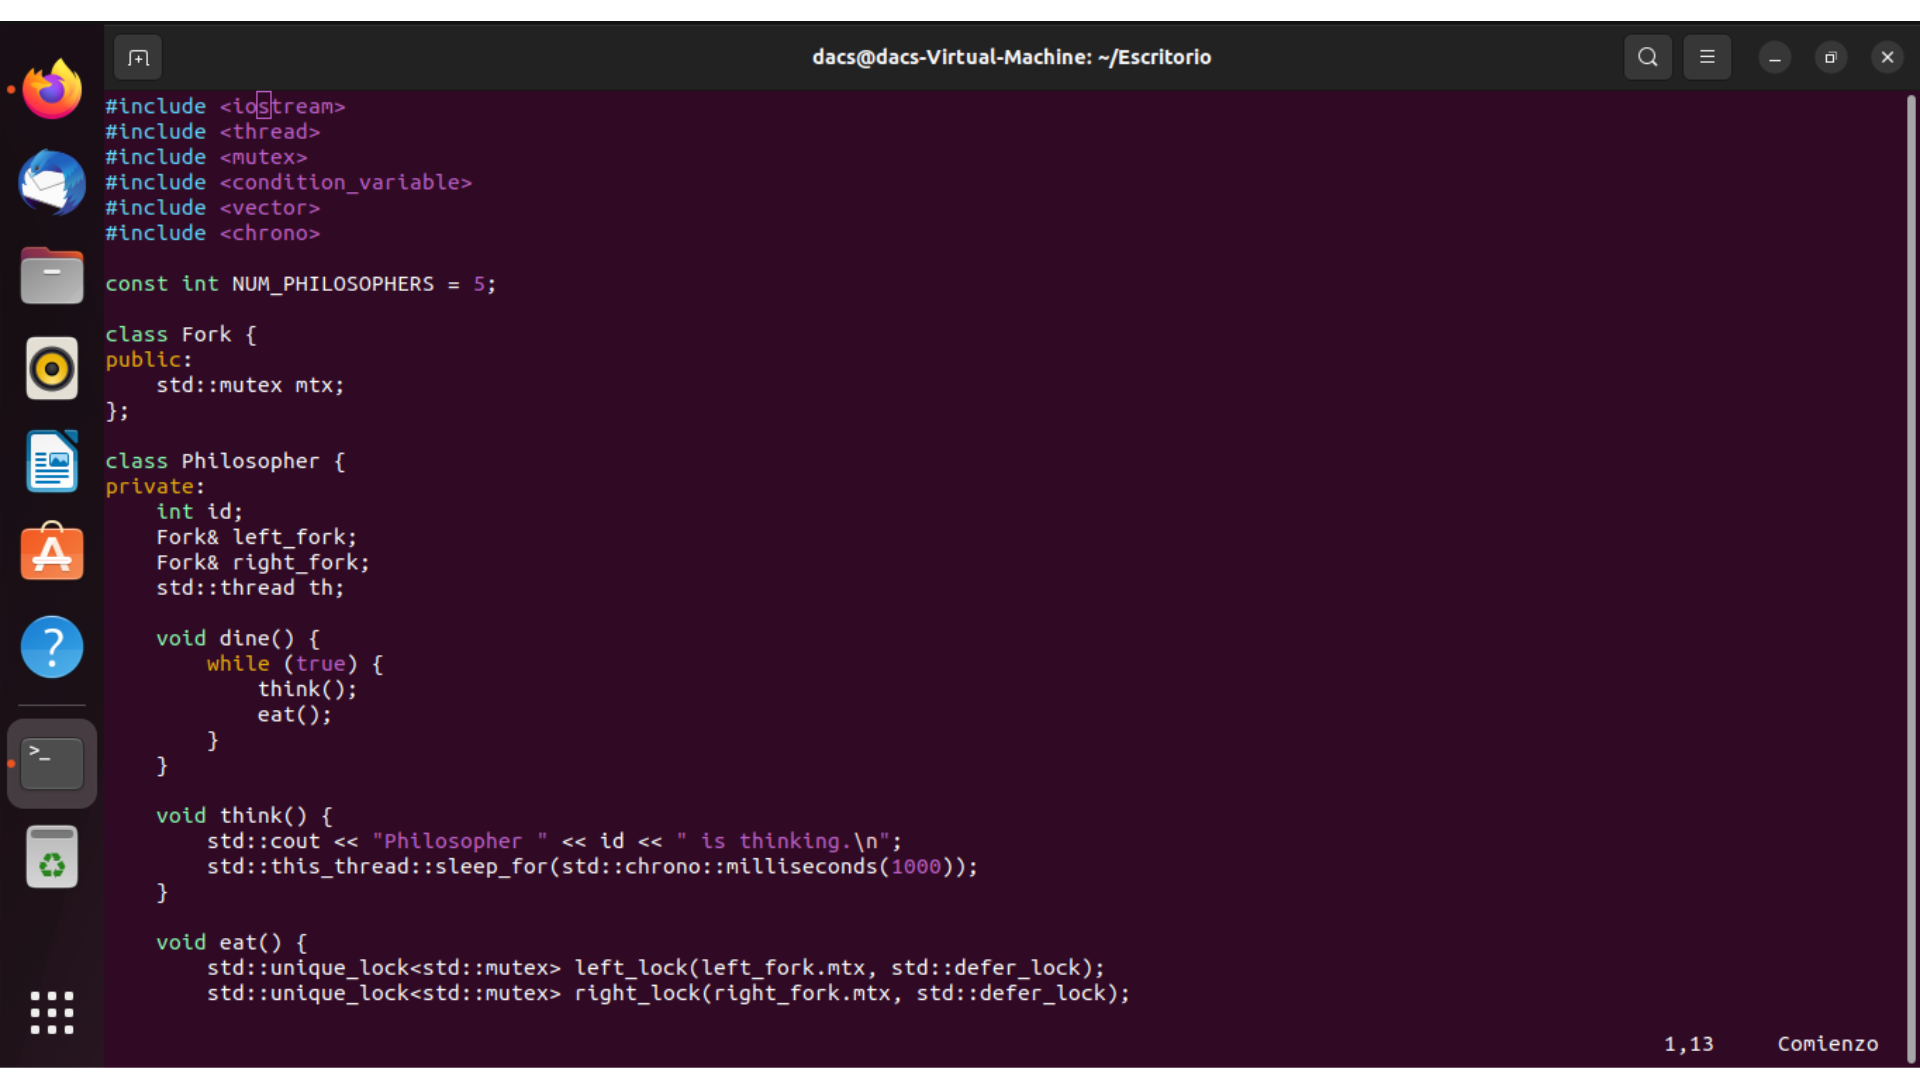
\includegraphics[width=0.3\textwidth]{Hyper-V/8.png}
  \caption{Codificación con Vim en Ubuntu}
\end{figure}

\begin{figure}[htbp]
  \centering
  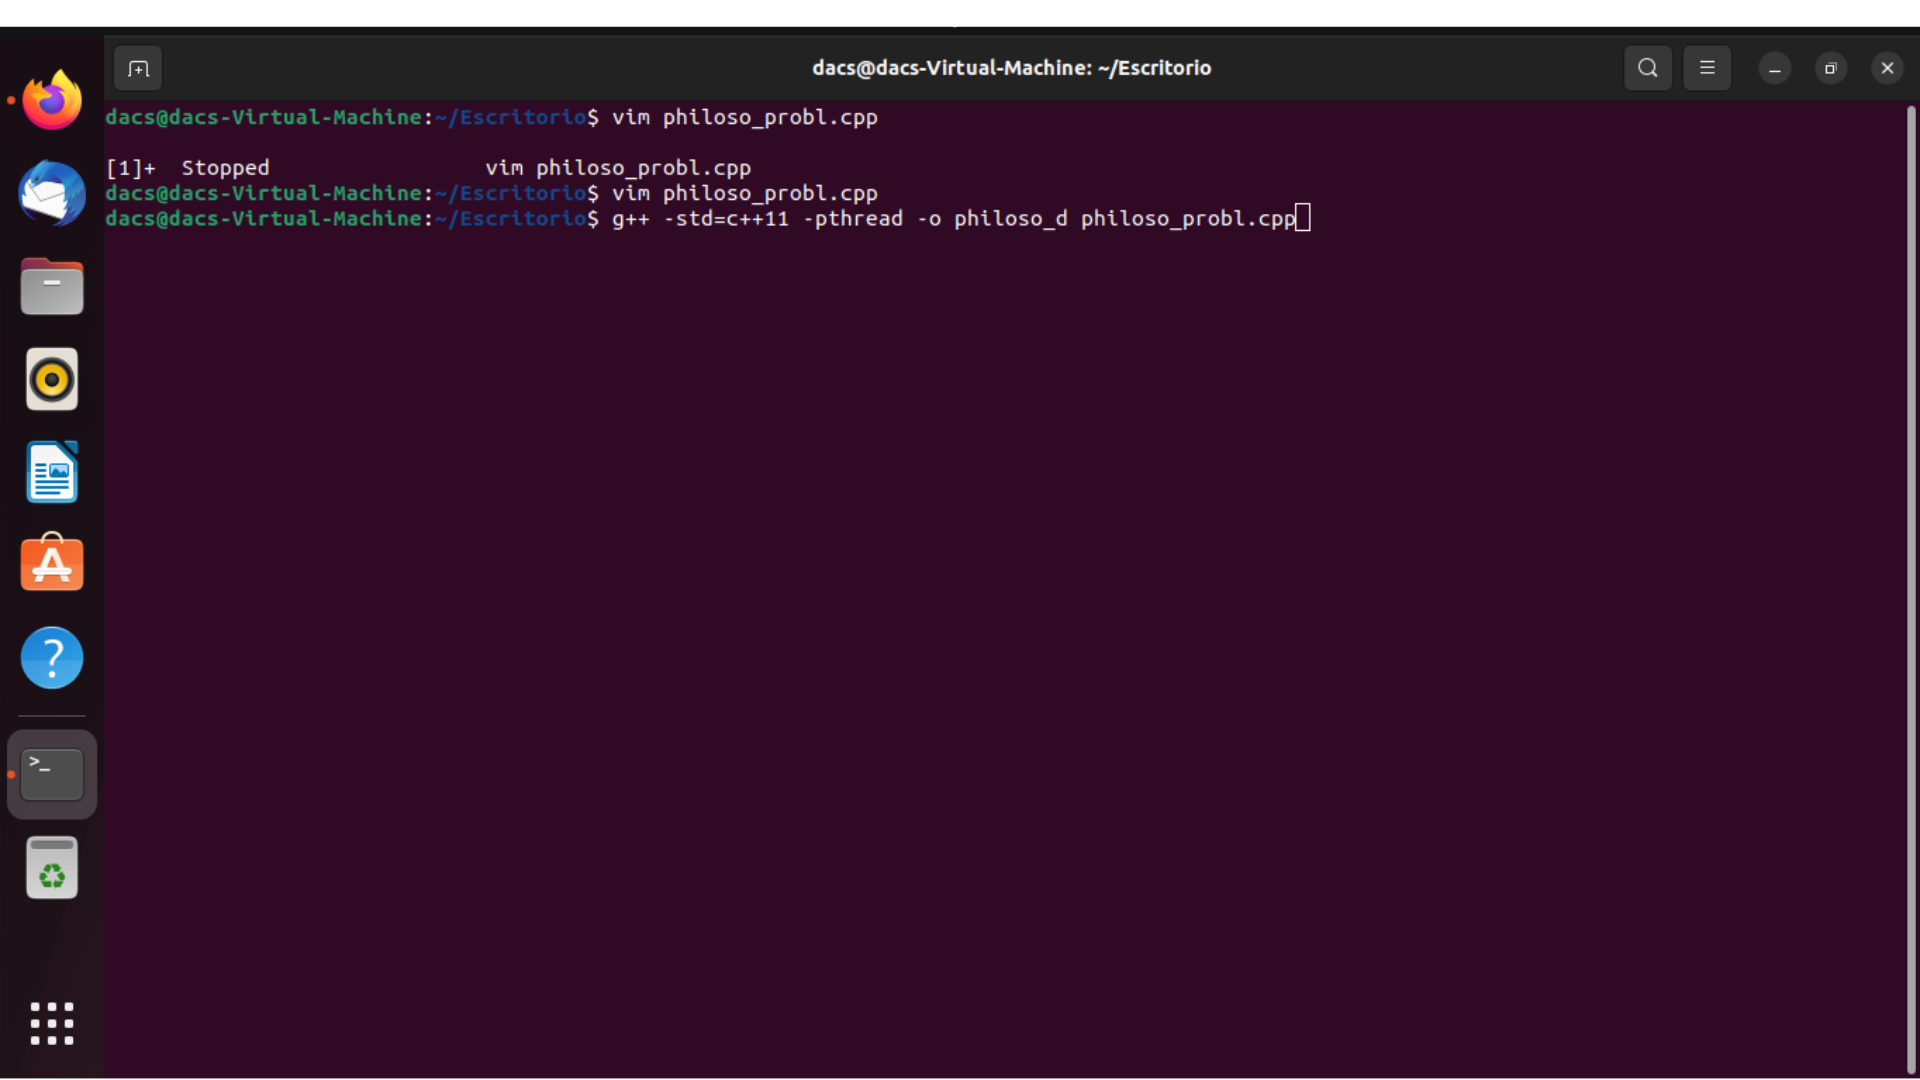
\includegraphics[width=0.3\textwidth]{Hyper-V/9.png}
  \caption{Compilación del código con g++}
\end{figure}

\begin{figure}[htbp]
  \centering
  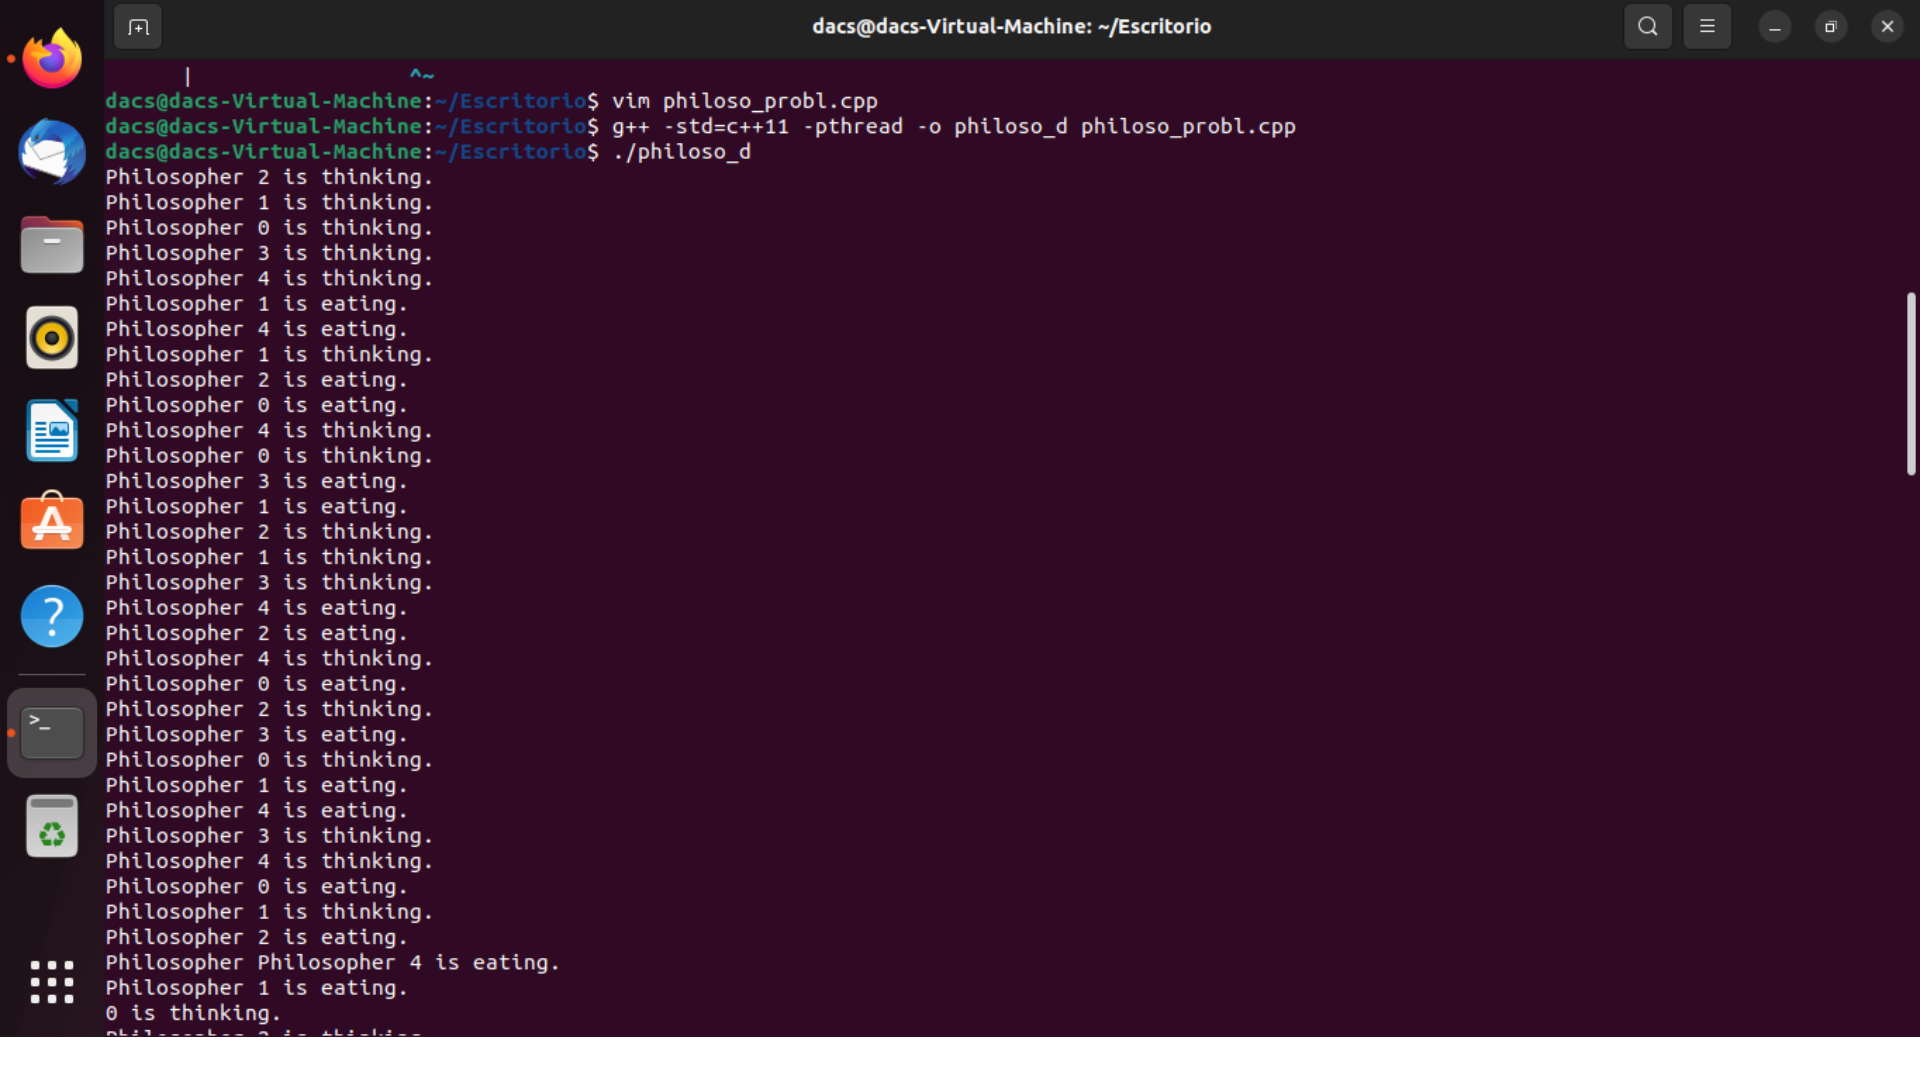
\includegraphics[width=0.3\textwidth]{Hyper-V/10.png}
  \caption{Ejecución de código y prueba}
\end{figure}


\FloatBarrier %Evita que una figura se salga de una sección asignada

Por último, dentro de nuestras pruebas tendremos la comprobación del GUI de nuestra maquina virtual, ejecutando una página web (GitHub) y luego un editor de Texto (Libre Office), esto para verificar si todas la funcionalidades del sistema operativo se mantienen adecuadas dentro de nuestro entorno de Hyper-V Server.\\

\begin{figure}[htbp]
  \centering
  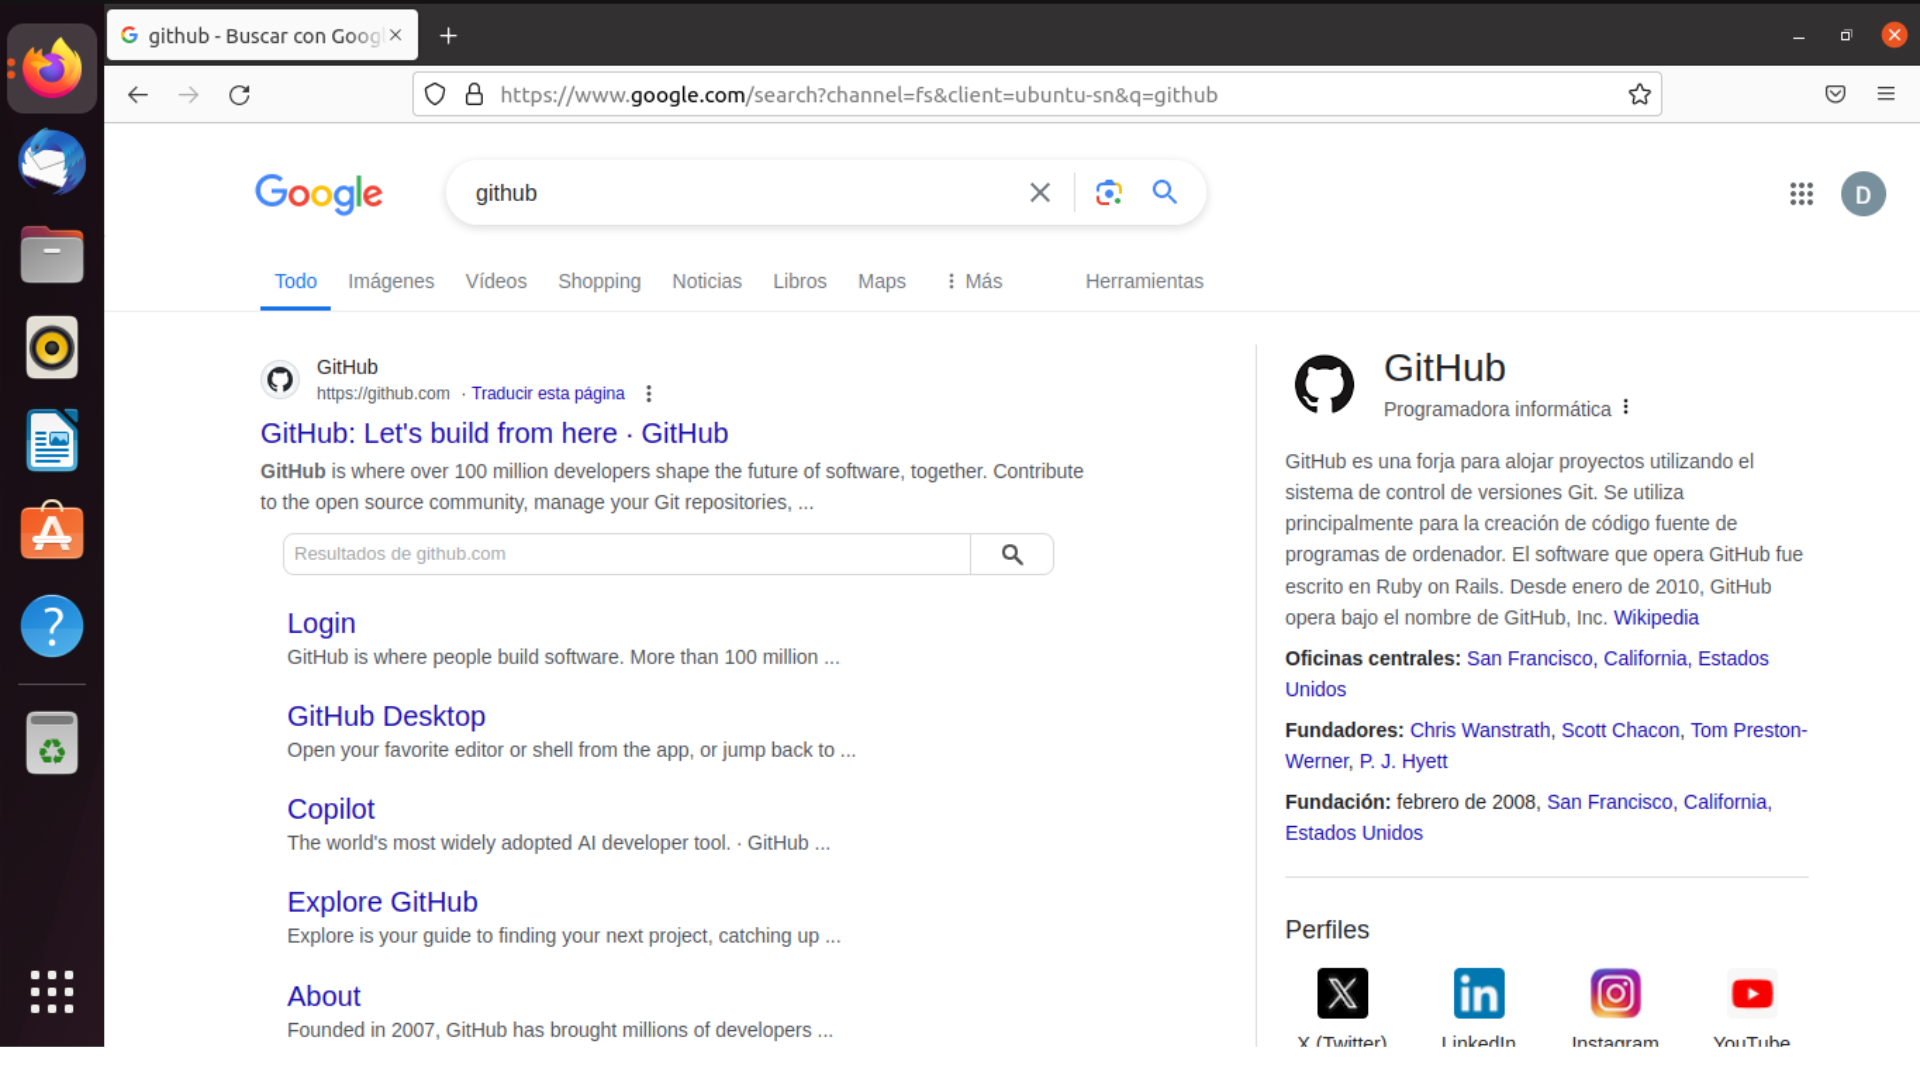
\includegraphics[width=0.3\textwidth]{Hyper-V/11.png}
  \caption{Prueba en navegador Firefox}
\end{figure}

\begin{figure}[htbp]
  \centering
  \includegraphics[width=0.3\textwidth]{Hyper-V/Instalación 20.png}
  \caption{Prueba con LibreOffice}
\end{figure}

\FloatBarrier %Evita que una figura se salga de una sección asignada

\subsection{Instalación de Microsoft Hyper-V Server}
Durante el proceso de instalación y ejecución de sistemas operativos en Microsoft Hyper-V Server, se destacó la facilidad y la interfaz amigable proporcionada por esta plataforma de virtualización. Este aspecto facilitó significativamente la instalación de Ubuntu, así como de otros sistemas operativos, permitiendo una configuración inicial rápida y eficiente del entorno de desarrollo requerido.\\
\begin{figure}[htbp]
  \centering
  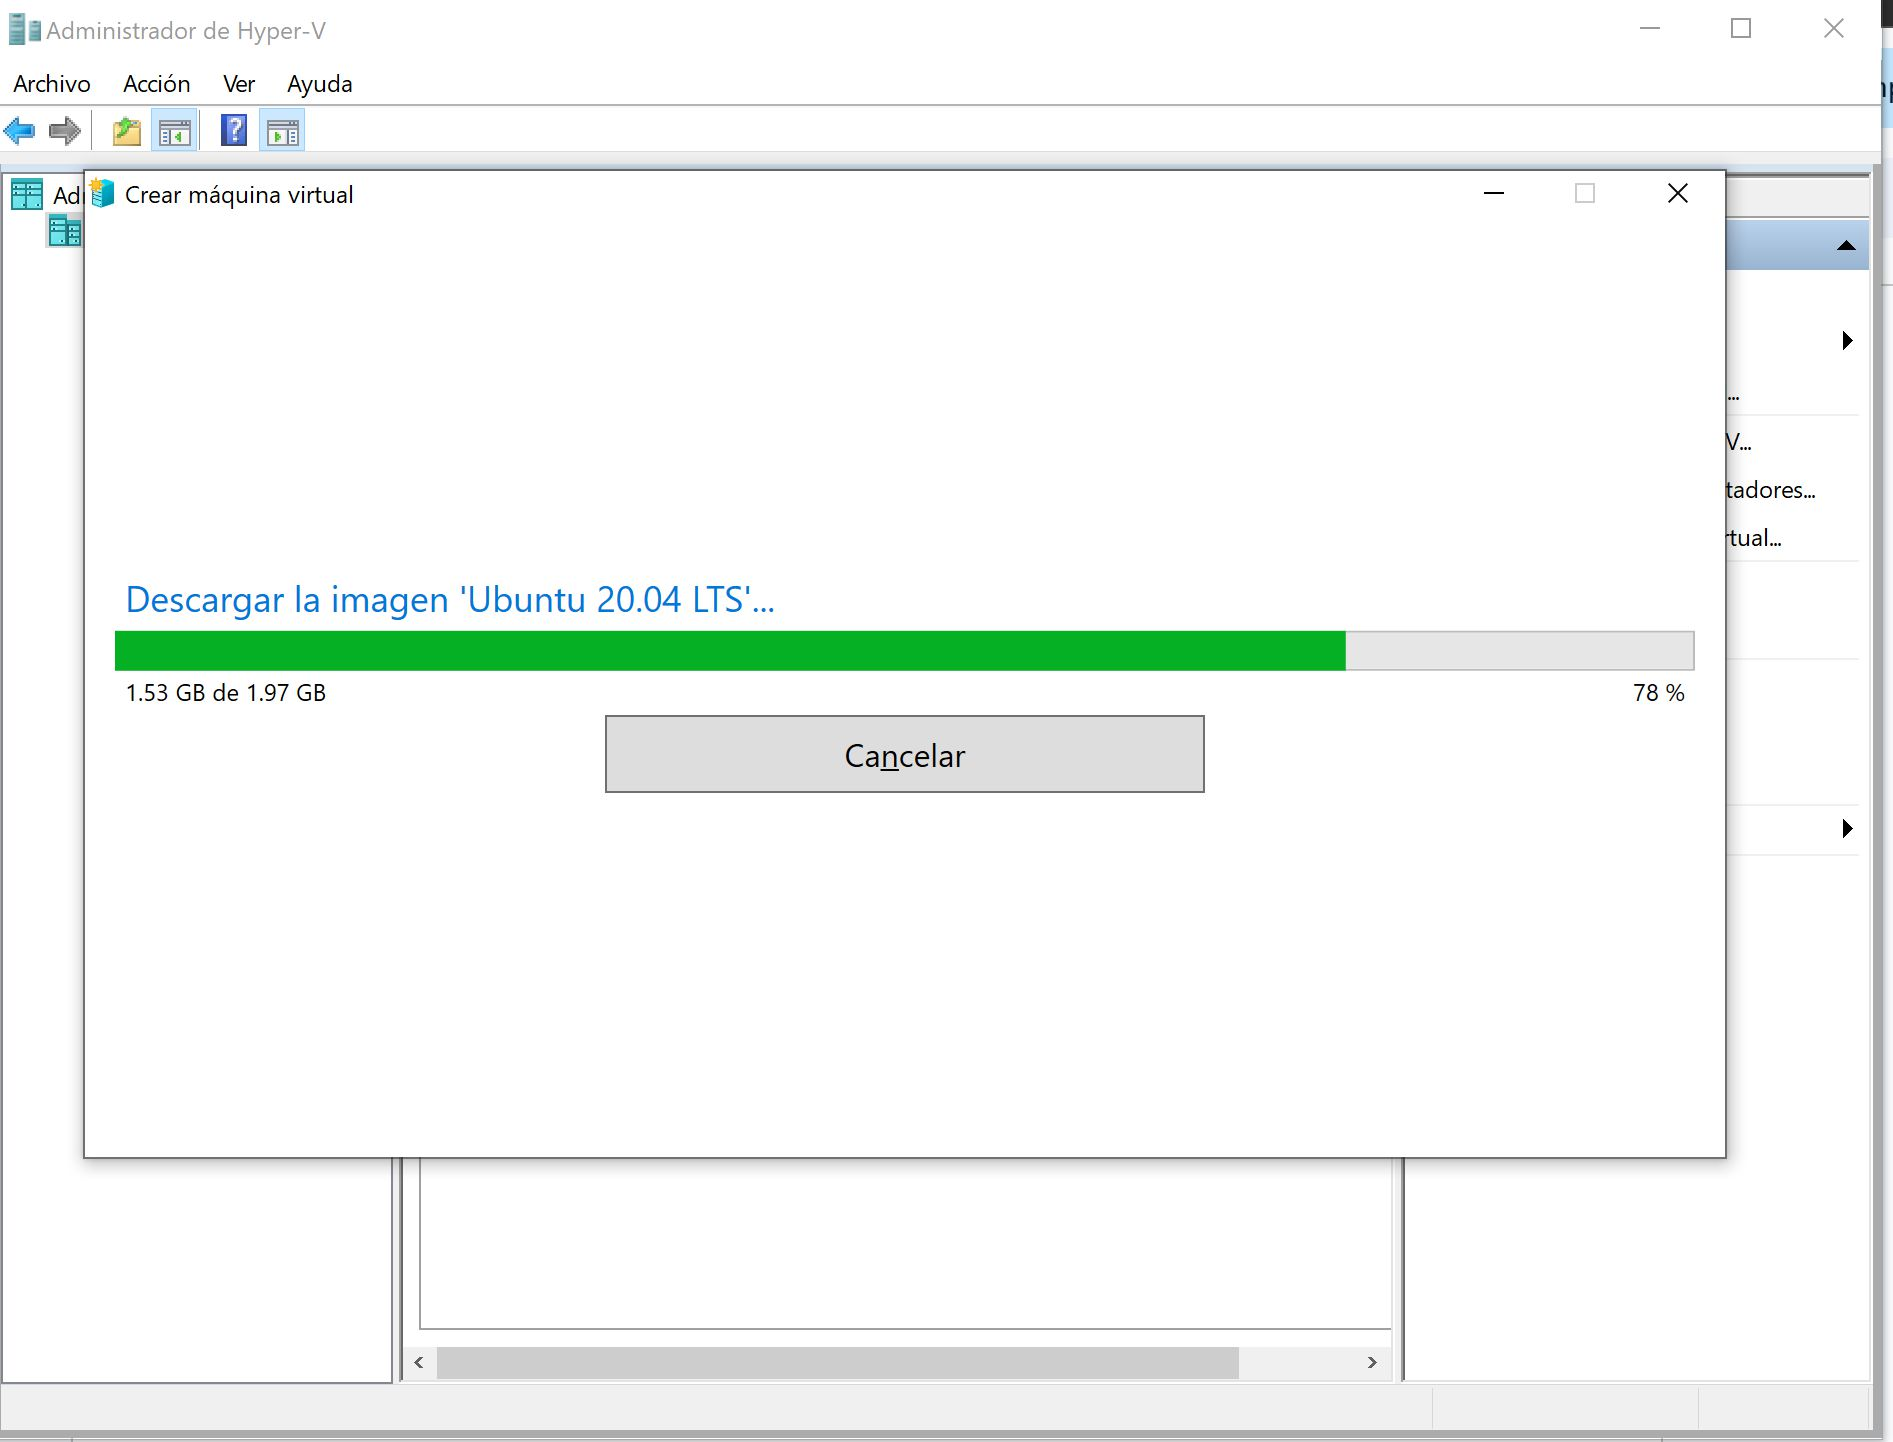
\includegraphics[width=0.3\textwidth]{enyel1.jpg}
  \caption{Descargando Ubuntu para Hyper-V}
\end{figure}
\begin{figure}[htbp]
  \centering
  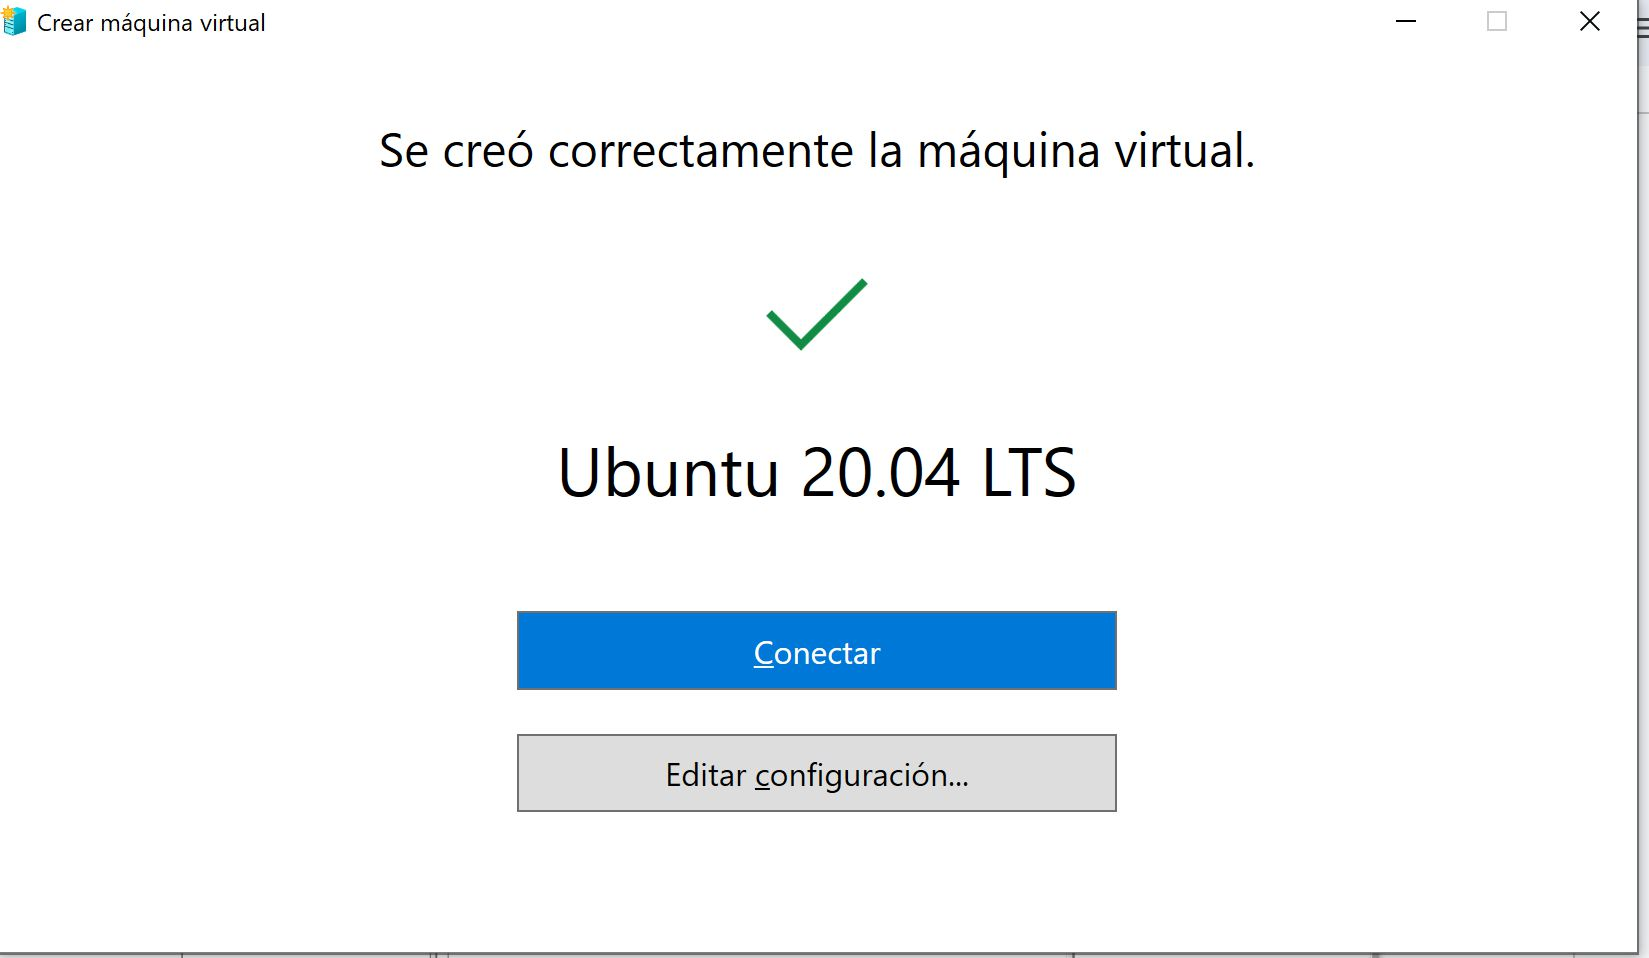
\includegraphics[width=0.3\textwidth]{enyel5.jpg}
  \caption{Creando maquina virtual}
\end{figure}
Al completar la creación rapida de la maquina virtual, seguiremos con su proceso de instalacion del propio sistema operativo.

\begin{figure}[htbp]
  \centering
  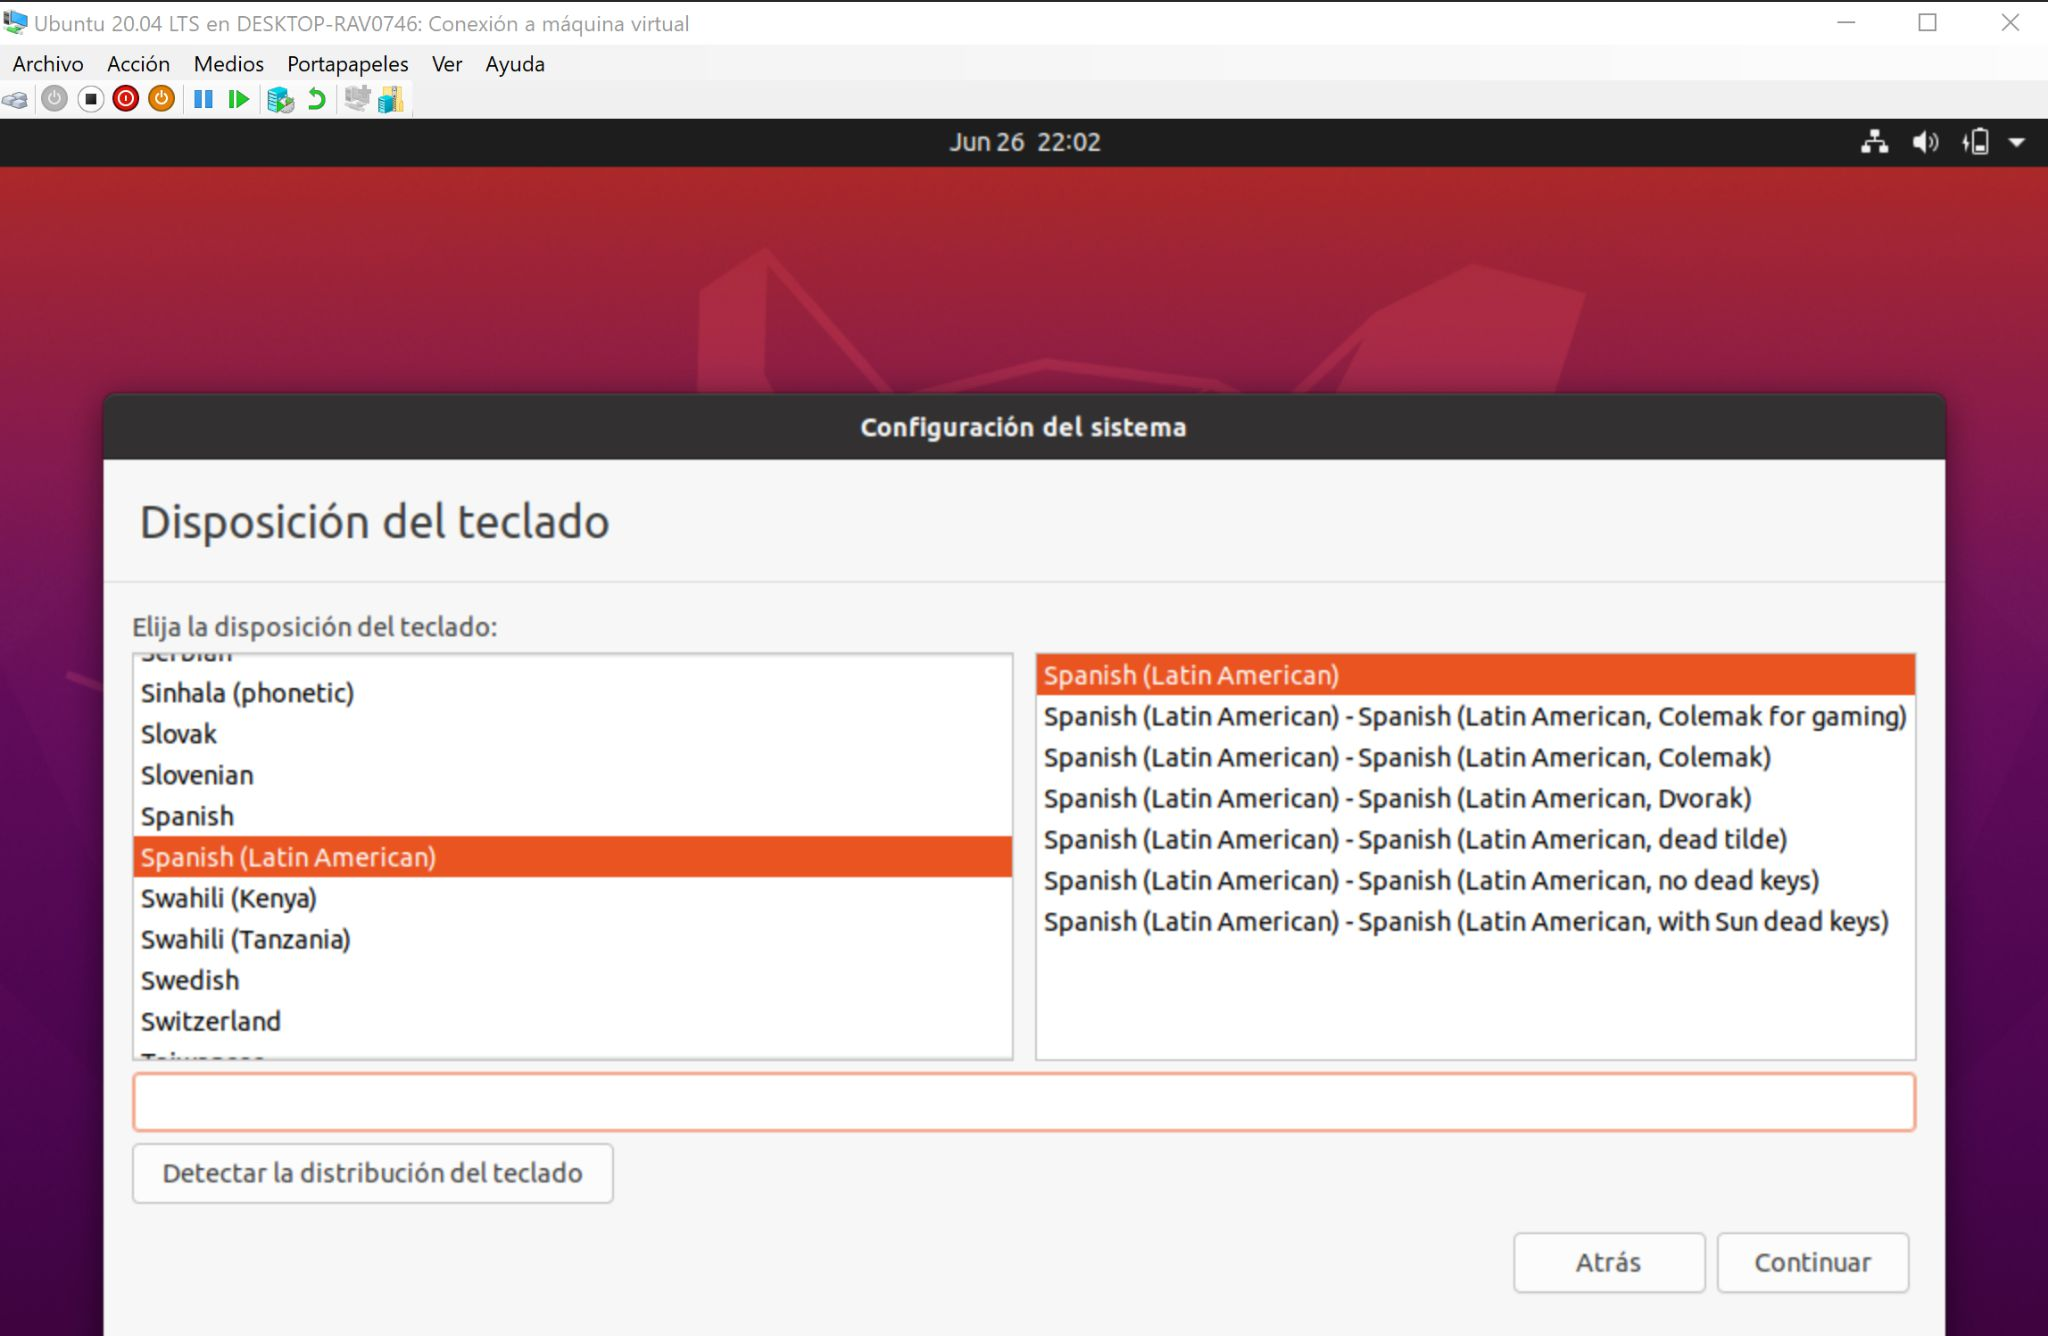
\includegraphics[width=0.3\textwidth]{enyel7.jpg}
  \caption{Configurando ubuntu}
\end{figure}
 Configuraremos ubuntu en el idioma y distribución de teclado que querramos.
\begin{figure}[htbp]
  \centering
  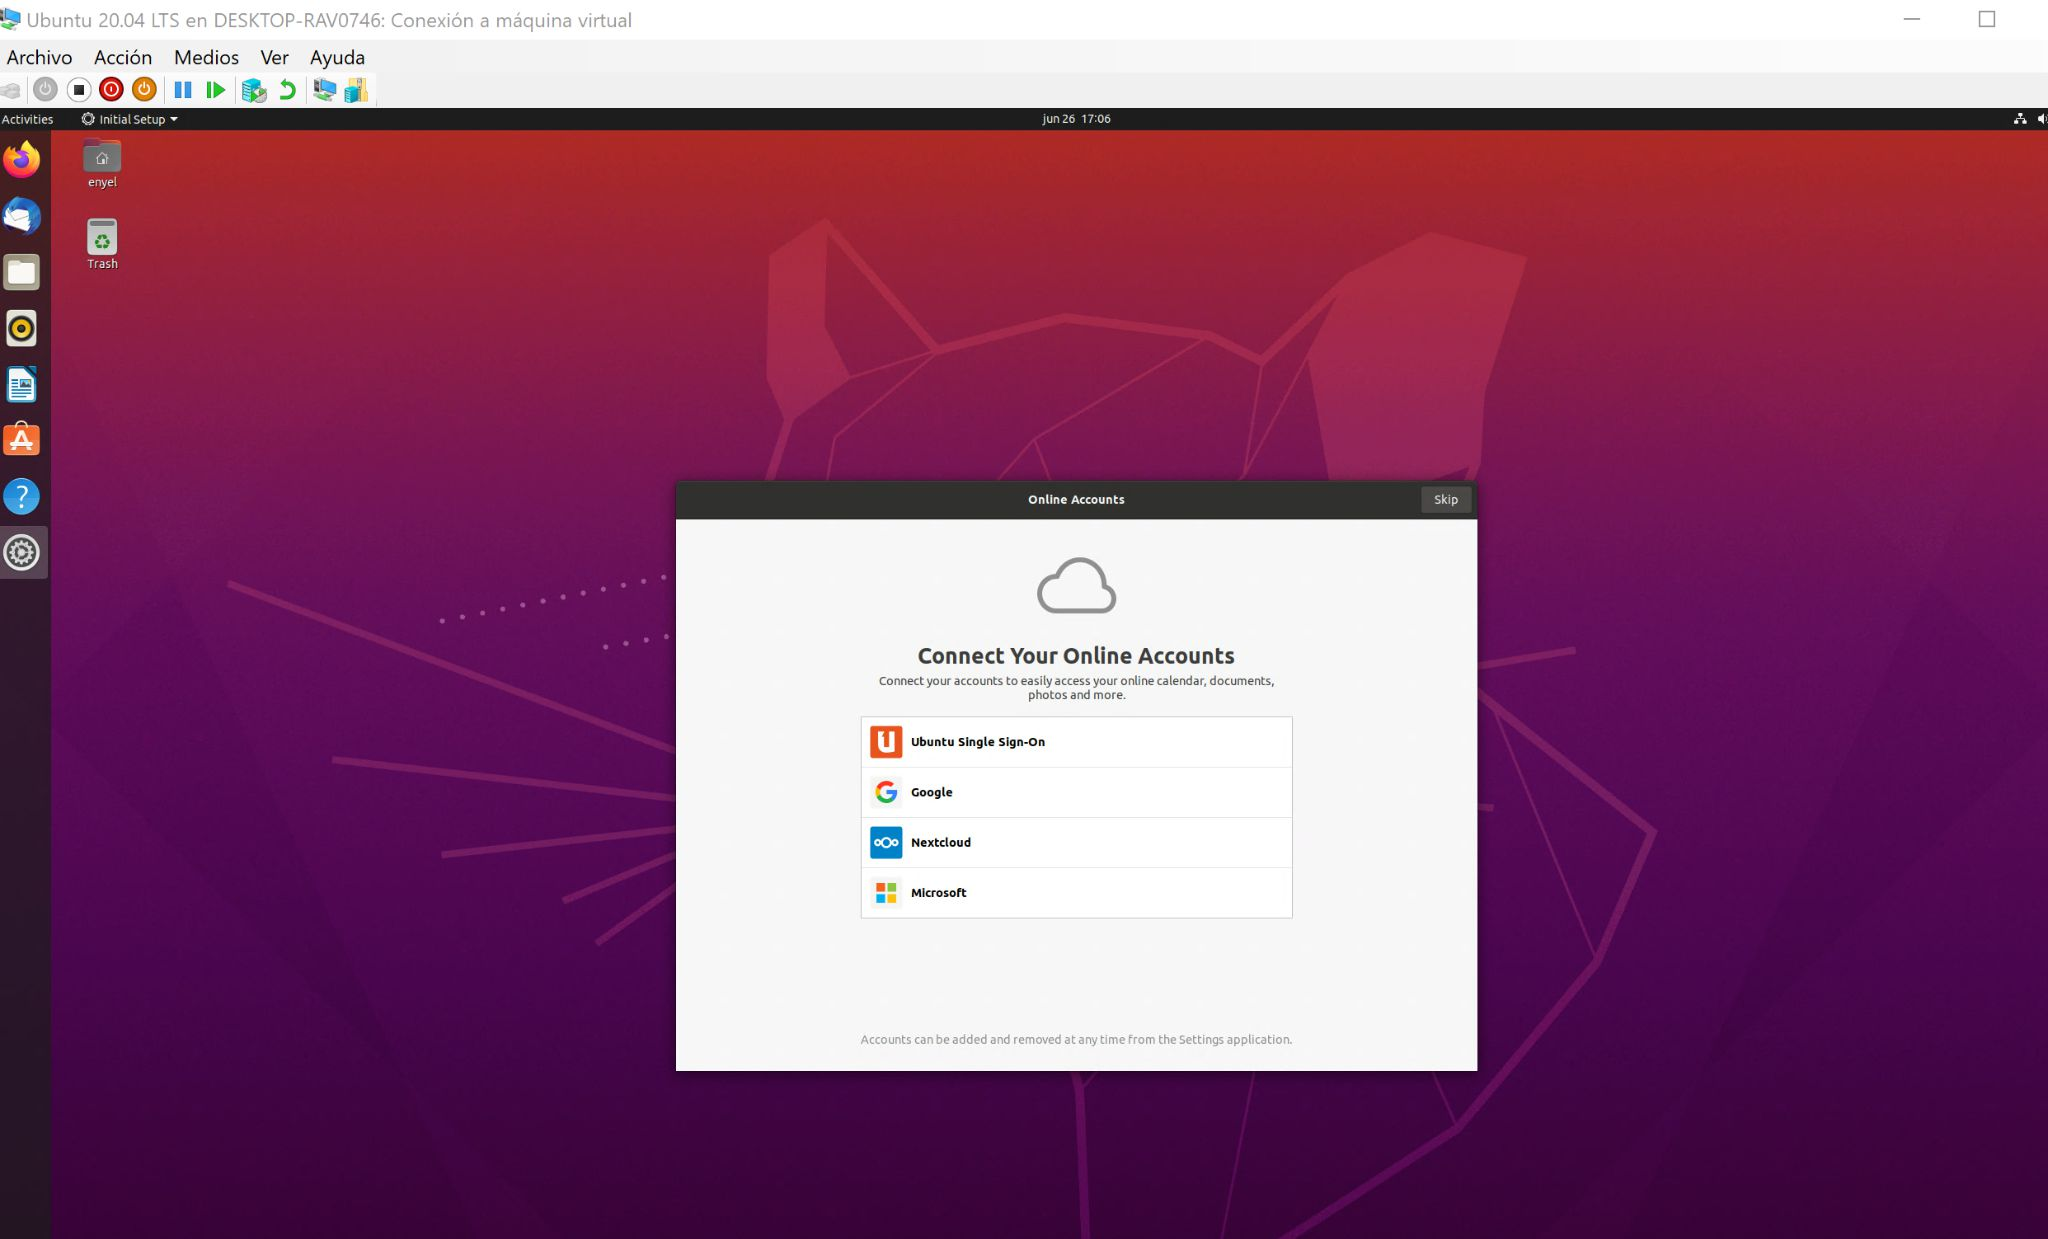
\includegraphics[width=0.3\textwidth]{enyel2.jpg}
  \caption{Escritorio de Ubuntu}
\end{figure}

\begin{figure}[htbp]
  \centering
  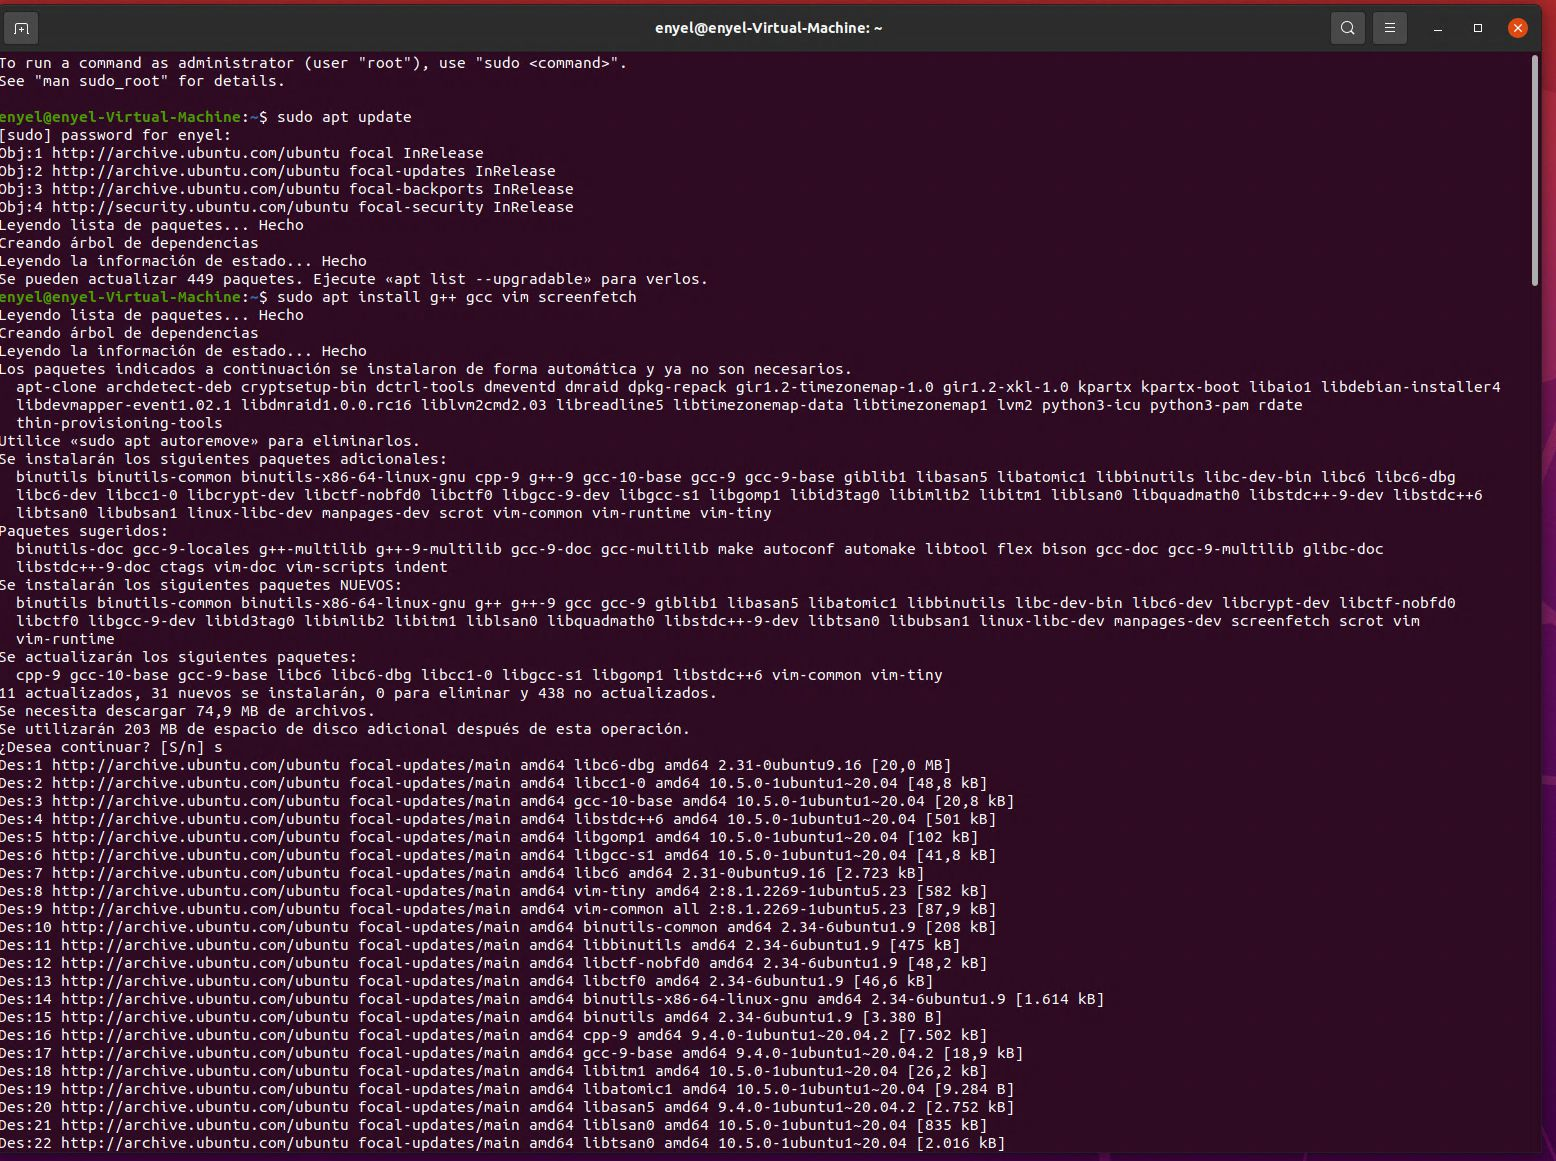
\includegraphics[width=0.3\textwidth]{enyel3.jpg}
  \caption{Instalando g++ gcc vim y screenfetch}

  \centering
  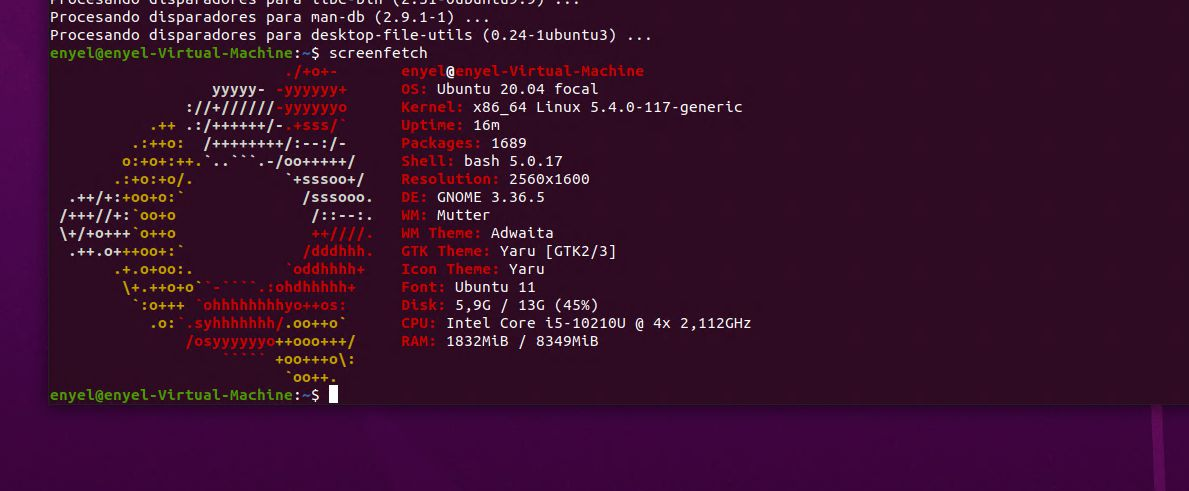
\includegraphics[width=0.3\textwidth]{enyel4.jpg}
  \caption{ejecutando screenfetch}


  \centering
  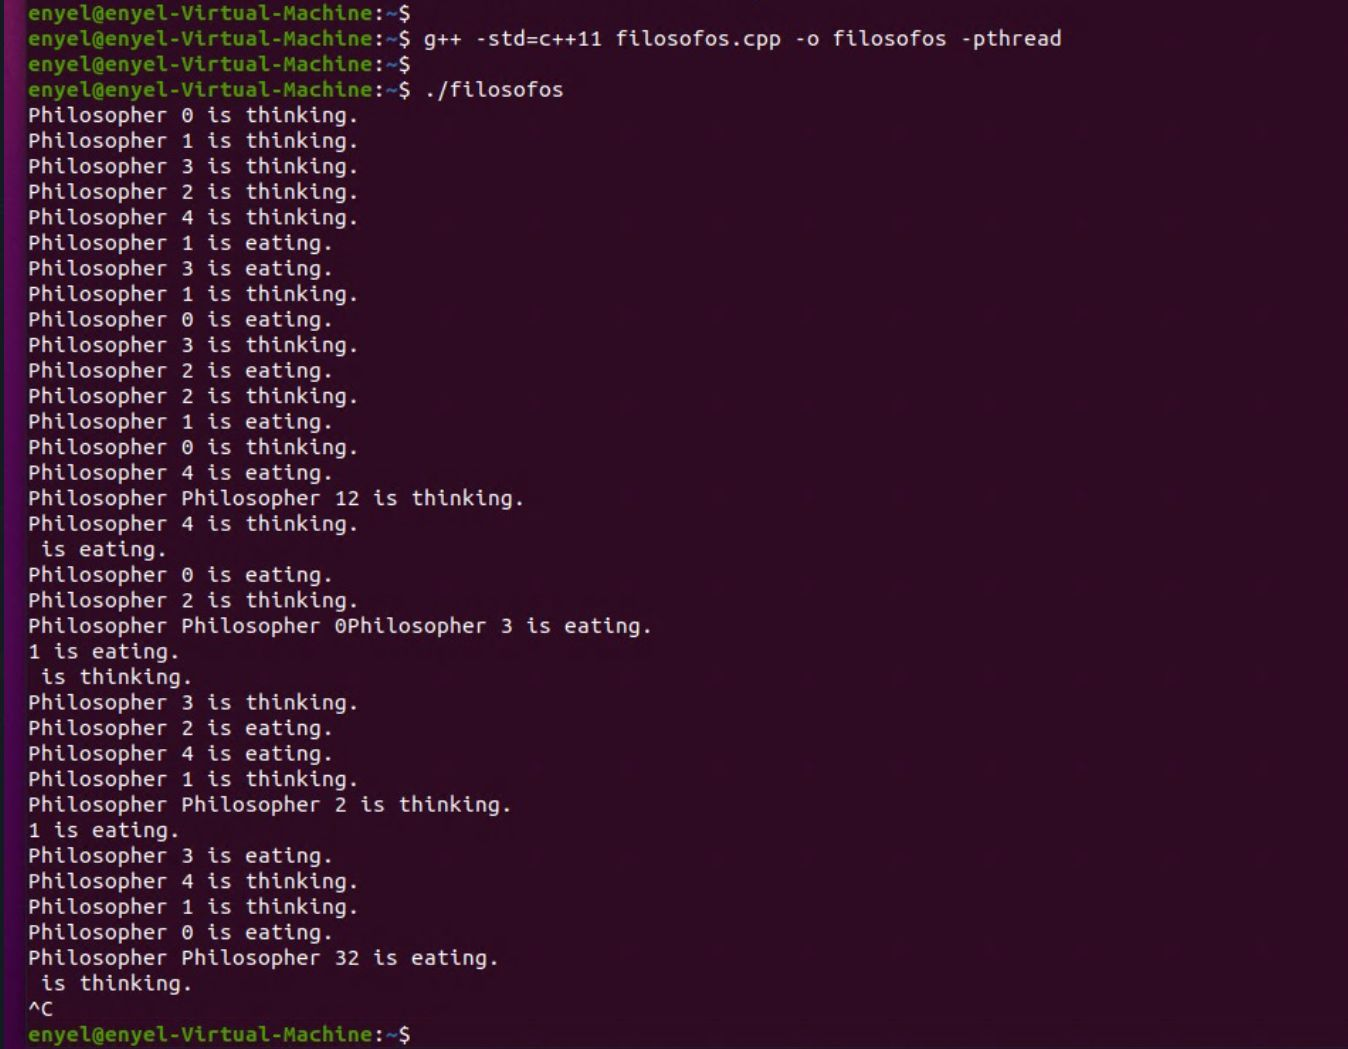
\includegraphics[width=0.3\textwidth]{enyel8.jpg}
  \caption{ejecutando cena de filosofos}
\end{figure}

\FloatBarrier %Evita que una figura se salga de una sección asignada

\subsection{Integración con Windows y otros sistemas de virtualización}
\begin{itemize}
    \item \textbf{Hyper-V}: Profunda integración con el ecosistema de Windows, ideal para entornos empresariales que ya utilizan infraestructura de Microsoft.
    \item \textbf{VMware/VirtualBox}: Son hipervisores de terceros que se instalan adicionalmente. VMware es ampliamente utilizado en entornos empresariales y soporta una variedad de sistemas operativos anfitriones. VirtualBox es gratuito y soporta múltiples sistemas operativos anfitriones.
\end{itemize}

\subsection{Rendimiento y Escalabilidad de Microsoft Hyper-V Server}
\begin{itemize}
    \item \textbf{Hyper-V}: Excelente rendimiento en entornos de Windows, con soporte para características avanzadas como la replicación de VM (Hyper-V Replica) y alta disponibilidad (Failover Clustering).
    \item \textbf{VMware}: Reconocido por su rendimiento y escalabilidad superior en grandes centros de datos, con características avanzadas de gestión y automatización (vSphere, vMotion).
    \item \textbf{VirtualBox}: Buen rendimiento para uso personal y desarrollo, pero no está diseñado para entornos de producción a gran escala.
\end{itemize}

\section{Conclusiones}
\subsection{Microsoft Hyper-V Server:}
\subsubsection{Eficiencia y Flexibilidad}
Hyper-V permite ejecutar varios sistemas operativos en un solo servidor fisico dando flexibilidad para adaptarse a muchas necesidades. Tambien rescatar las caracteristicas avanzadas como Live Migration y Hyper-V Replica porque ayudan significativamente la eficiencia de las operaciones.
\subsubsection{Rentabilidad}
Hyper-V es un software gratuito que se centra completamente a la virtualizacion ofreciendonos varias herramientas, aunque tambien hay una version de paga que es mas completa.
\subsubsection{Compatibilidad}
Hyper-V tiene una amplia compatibilidad con diferentes sistemas operativos de Windows y Linux y tambien posee compatibilidad con algunas aplicaciones.\\

Como se detalló anteriormente, Hyper V Manager es una herramienta importante.Sus amplias funcionalidades, junto con sus requisitos accesibles y beneficios claros, lo convierten en una opción funcional y fexible.

\subsection{Hyper V Manager:}

\subsubsection{Eficiencia}
Una de las ventajas más significativas de Hyper-V Manager es su capacidad para maximizar la eficiencia del hardware. Al permitir la creación y gestión de múltiples máquinas virtuales en un solo sistema físico. Esta consolidación no solo ahorra en costos de hardware, sino también en espacio, energía y enfriamiento, lo cual es crucial para la sostenibilidad y eficiencia operativa de las organizaciones.

\subsubsection{Seguridad}
Hyper-V Manager ofrece un aislamiento completo entre las máquinas virtuales, lo que mejora significativamente la seguridad. Cada maquina virtual opera de manera independiente, minimizando el riesgo de que una vulnerabilidad en una de ellas comprometa el sistema entero.

\subsubsection{Escalabilidad y flexibilidad}
Los administradores pueden ajustar rápidamente la cantidad de recursos asignados a cada maquina virtual, permitiendo un crecimiento ágil y adaptado a las demandas cambiantes. Esta flexibilidad es especialmente útil en entornos de desarrollo y pruebas, donde se requiere crear y destruir entornos rápidamente para experimentar y validar nuevas soluciones.

\section{Recomendaciones}
\subsection{Evaluacion Inicial}
Antes de querer implementar Hyper-V en tu máquina, primeramente hay que verificar los requisitos, tanto de software como los de hardware para garantizar un desempeño óptimo
\subsection{Capacitacion}
Aunque parezca sencillo entender los conceptos basicos de Hyper-V consideramos que seria muy bueno optar por algunas capacitaciones sobre la administracion y configuracion de Hyper-V Server para maximizar los beneficios y minimizar los problemas operativos
\subsection{Monitoreo continuo}
El poder utilizar algunas herramientas de monitoreo para supervisar el rendimiento y la seguridad del entorno de Hyper-V nos aseguran que se pueda tomar medidas mas rapidas ante algun problema que ocurra.
% Bibliografía
\bibliographystyle{IEEEtran}
\bibliography{citas} % Nombre del archivo .bib donde tienes las referencias

\end{document}
